% Here you insert the stuff that comes before the preface
% Each preface section is contained in a \prefacesection and starts on a
% new page.  These are numbered using Roman numerals.
% If there are no such pages, do not remove the \beforepreface command
% since it creates the title page.	
\beforepreface

% Abstract
\prefacesection{Abstract}

Diabetes is difficult to manage in a patient's daily routine as it involves managing one’s glucose levels within prescribed bounds. These levels are influenced by a variety of factors that are hard to keep track off on daily basis including sleep, diet, exercise, and stress.

The Diabetes Analytic and Recommendations Engine (DARE) was developed to help diabetic patients intuitively manage their glucose levels and receive recommendations to ensure they maintain their glucose levels within their prescribed bounds.  DARE is made up of two docker containerized components: Predictions Engine and Recommendations Engine.

The Predictions Engine is responsible for surveying past glucose level data to predict the glucose level for the prescribed time window (i.e. the next hour, 5 hours, or a day). This predicted glucose value is then channeled to the Recommendations Engine which is responsible for collecting any additional information on factors that impact glucose levels such as diet, stress, sleep, and exercise. Such factors can be retrieved using device health APIs and other smart Internet of Things (IOT) or through smart assistants such as Amazon Alexa. The Recommendations Engine then uses a correlation matrix to identify the most applicable recommendation and sends it to the user through a React Native application.

The system architecture was designed around the Service-Oriented Architecture pattern wherein each unit serves a distinctive function. Containerization enables modularity across the system and scalability using tools like Kubernetes for cluster-based scaling. It also enables independent deployment of each unit and permits third-party entities to integrate a service within their own technologies without requiring dependencies on the rest of the system components.

% Acknowledgements
\prefacesection{Acknowledgements}
We would like to express our sincere gratitude to Dr. Zied Boudia and Dr. Mohamed IbnKahla for their continuous positive feedback throughout the year, and for always pushing us forward to fulfill this milestone. Additionally, we would like to thank Kareem Arab, Abdallah Jarwan and Arslan Ahmed for their valuable help in answering the various project-related questions that we had throughout the year. Lastly, we would like to thank Anasstassia Gharib for recommending our team at the beginning of the year to work on this project. 


% Contents References
\prefaceTOC   % Print the Table of Contents
\prefaceLOF   % Print the List of Figures
\prefaceLOT   % Print the List of Tables

\prefacesection{List of Abbreviations}
\begin{tabular}[t]{l@{\hspace*{2cm}}l}
	API & Application Program Interface \\
	APP & Application \\
	CHEO & Children's Hospital of Eastern Ontario \\
	DARE & Diabetes Analytics and Recommendation Engine \\
	EDS & Error Difference Square \\
	EDST & Error Difference Square Total \\
	GL & Glucose Level \\
	HIPAA & Health Insurance Portability and Accountability Act \\
	IOT & Internet of Things \\
	NRC & National Research Council \\
	PE & Prediction Engine \\
	RE & Recommendation Engine \\
	RESTful & Representational State Transfer \\
	RFR & Random Forest Regression \\
	SETI & Search for Extra Terrestrial Intelligence \\
	SLR & Simple Linear Regression \\
	SOA & System-Oriented Architecture \\
	SVR & Support Vector Regression \\
	T2DM & Type 2 Diabetes Mellitus 	\\
	WLR & Weight Linear Regression \\
	RNN & Recurrent Neural Network \\
	FFNN & Feed Forward Neural Network \\
	LSTN & Long-Short Term Memory\\
\end{tabular}

\endpreface
	

\chapter{Introduction}
\label{cha:introduction}
% Begin Chapter
Type 2 Diabetes Mellitus (T2DM) is increasing at an alarming rate across Canada, affecting millions of individuals and their families and contributing to the ever-increasing health-care costs \cite{1}. 
In 2017, 7.3 percent of Canadians aged 12 and older (roughly 2.3 million people) reported being diagnosed with diabetes \cite{2}. Between 2016 and 2017, the proportion of males who reported being diagnosed with diabetes increased from 7.6 percent in 2016 to 8.4 percent in 2017 whereas, the proportion of females remained consistent between the two years \cite{2}. It is estimated that patients spend between 1,000 and 15,000 dollars a year on products such as test strips and medication \cite{1}. These costly expenses have forced some patients to abandon aggressive treatment, and as a result they end up costing the public health system, since such decisions could lead to expensive complications and even more expensive medication costs \cite{1}.
Diabetes is a lifelong condition which occurs when the body does not produce enough insulin, or when the insulin produced is not used effectively \cite{3}. Insulin is a hormone that helps the body control the level of sugar in the blood \cite{3}.
Consequently, glucose builds up in the blood instead of being used for energy[2]. If this condition is left unmanaged, the excess sugar in the blood can eventually cause problems \cite{3}. These problem could include a reduced quality of life as well as complications such as heart diseases, strokes and kidney diseases \cite{3}. 

\section{Motivation}
\label{sec:motivation}
% Begin Section
Being diagnosed with T2DM and having to manage the condition is not simple. It is important to note though that one can live a long and healthy life by keeping their blood sugar levels in the target range set by the patient and their health-care provider as well as managing one's lifestyle factors \cite{1}.
Over time, high blood sugar levels can cause complications. Fortunately, good diabetes care and management can prevent or delay the onset of these complications \cite{1}.
For this reason, Diabetes Analytics and Recommendation Engine (DARE) has been created with the intention of helping diabetes type II patients better self-manage their disease and consequently reduce the health care expenditure on diabetes. 

% End Section

\section{Competitors}
\label{sec:competitors}
% Begin Section
The idea of self-managing diabetes is not a new one on the digital market. A few companies have already launched applications that somehow share the general goal of DARE. 
The following is a discussion of both the similarities as well as the differences between these existing applications and DARE.
\bigbreak
\textbf{One Drop} is one application that tracks and analyzes a patient's blood sugar, medications, food and activity and then estimates future glucose values to provide food and activity suggestions based on a patient's current glucose level \cite{4}. However, ONEDROP differs from DARE in the sense that the data collected such as diet, stress and exercise is not harnessed for correlations in predicting glucose values but rather collected for tracking purposes only.
\bigbreak
\textbf{Glucose Buddy} is another application that tracks blood sugar, insulin, medication and food intake and gives a daily glucose level summary to the patient as well as predict the long term glucose trends \cite{5}. However, the application does not provide recommendation to the patient for disease management nor does it take lifestyle factors into consideration.
\bigbreak
\textbf{BlueStar} is a third application that provides personalized guidance based on glucose, medications, current health and a review of lifestyle factors \cite{6}. However, this application can only be used with a medical prescription, requires registration and is intended for use by patients who are at least 21 years old. 


% End Section

\section{Scope}
\label{sec:scope}
% Begin Section
Although there is no cure for diabetes, the condition can be managed by medication and/or insulin, as well as making healthy lifestyle choices. Therefore, DARE was developed to help youth and young adults with T2DM patients better manage their disease based on their past, current and predicted glucose levels as well as four lifestyle factors including sleep, diet, exercise and stress.

\subsection{Objectives}
\label{subsec:objectives}
% Begin Subsection
The following objectives were set for DARE to achieve the goals of this project:

\begin{itemize}
    \item \textbf{Data Analytics Engine:} implementing a data analytics engine capable of using current and historical data on glucose as well as the four lifestyle factors of sleep, diet, exercise and stress to predict glucose levels.
    \item \textbf{Correlation between Factors:} implementing a system capable of finding correlations between factors affecting glucose levels to make more accurate recommendations.
    \item \textbf{Recommendation Engine:} implementing a system capable of producing individualized and accurate recommendations based on the availability of data.
\end{itemize}

\begin{figure}[h!]
    \centering
    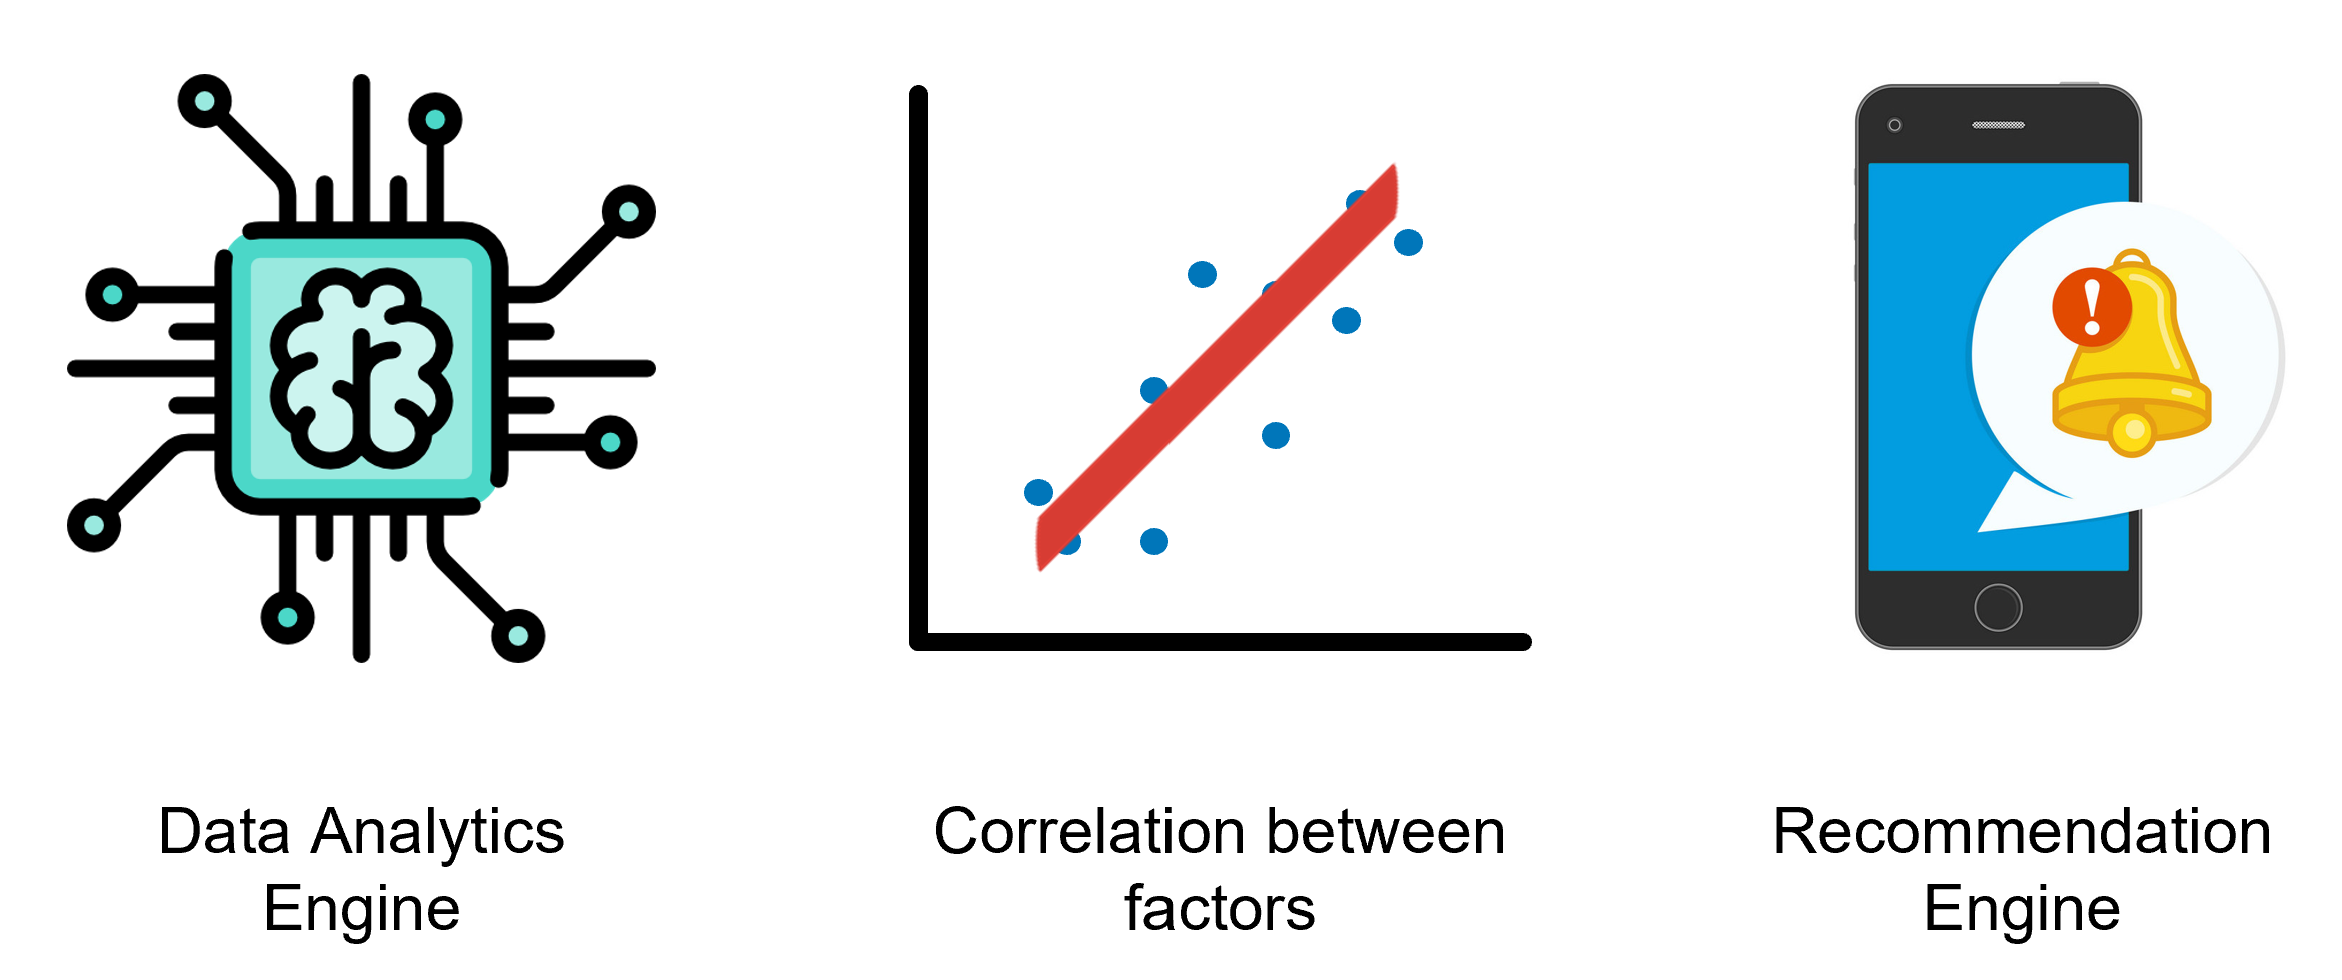
\includegraphics[width=\textwidth]{Figures/pooria/obj.png}
    \caption{Objectives of DARE}
\end{figure}

%%%%%%%%%%%%%%%%%%%%%%%%%%%%%%%%%%%%%%%%%%%%%%%%
%%%%                TEST                   %%%%%
%%%%%%%%%%%%%%%%%%%%%%%%%%%%%%%%%%%%%%%%%%%%%%%%
%\begin{figure}[h!]
%    \centering
%  \caption{TEST TEST TEST}
%  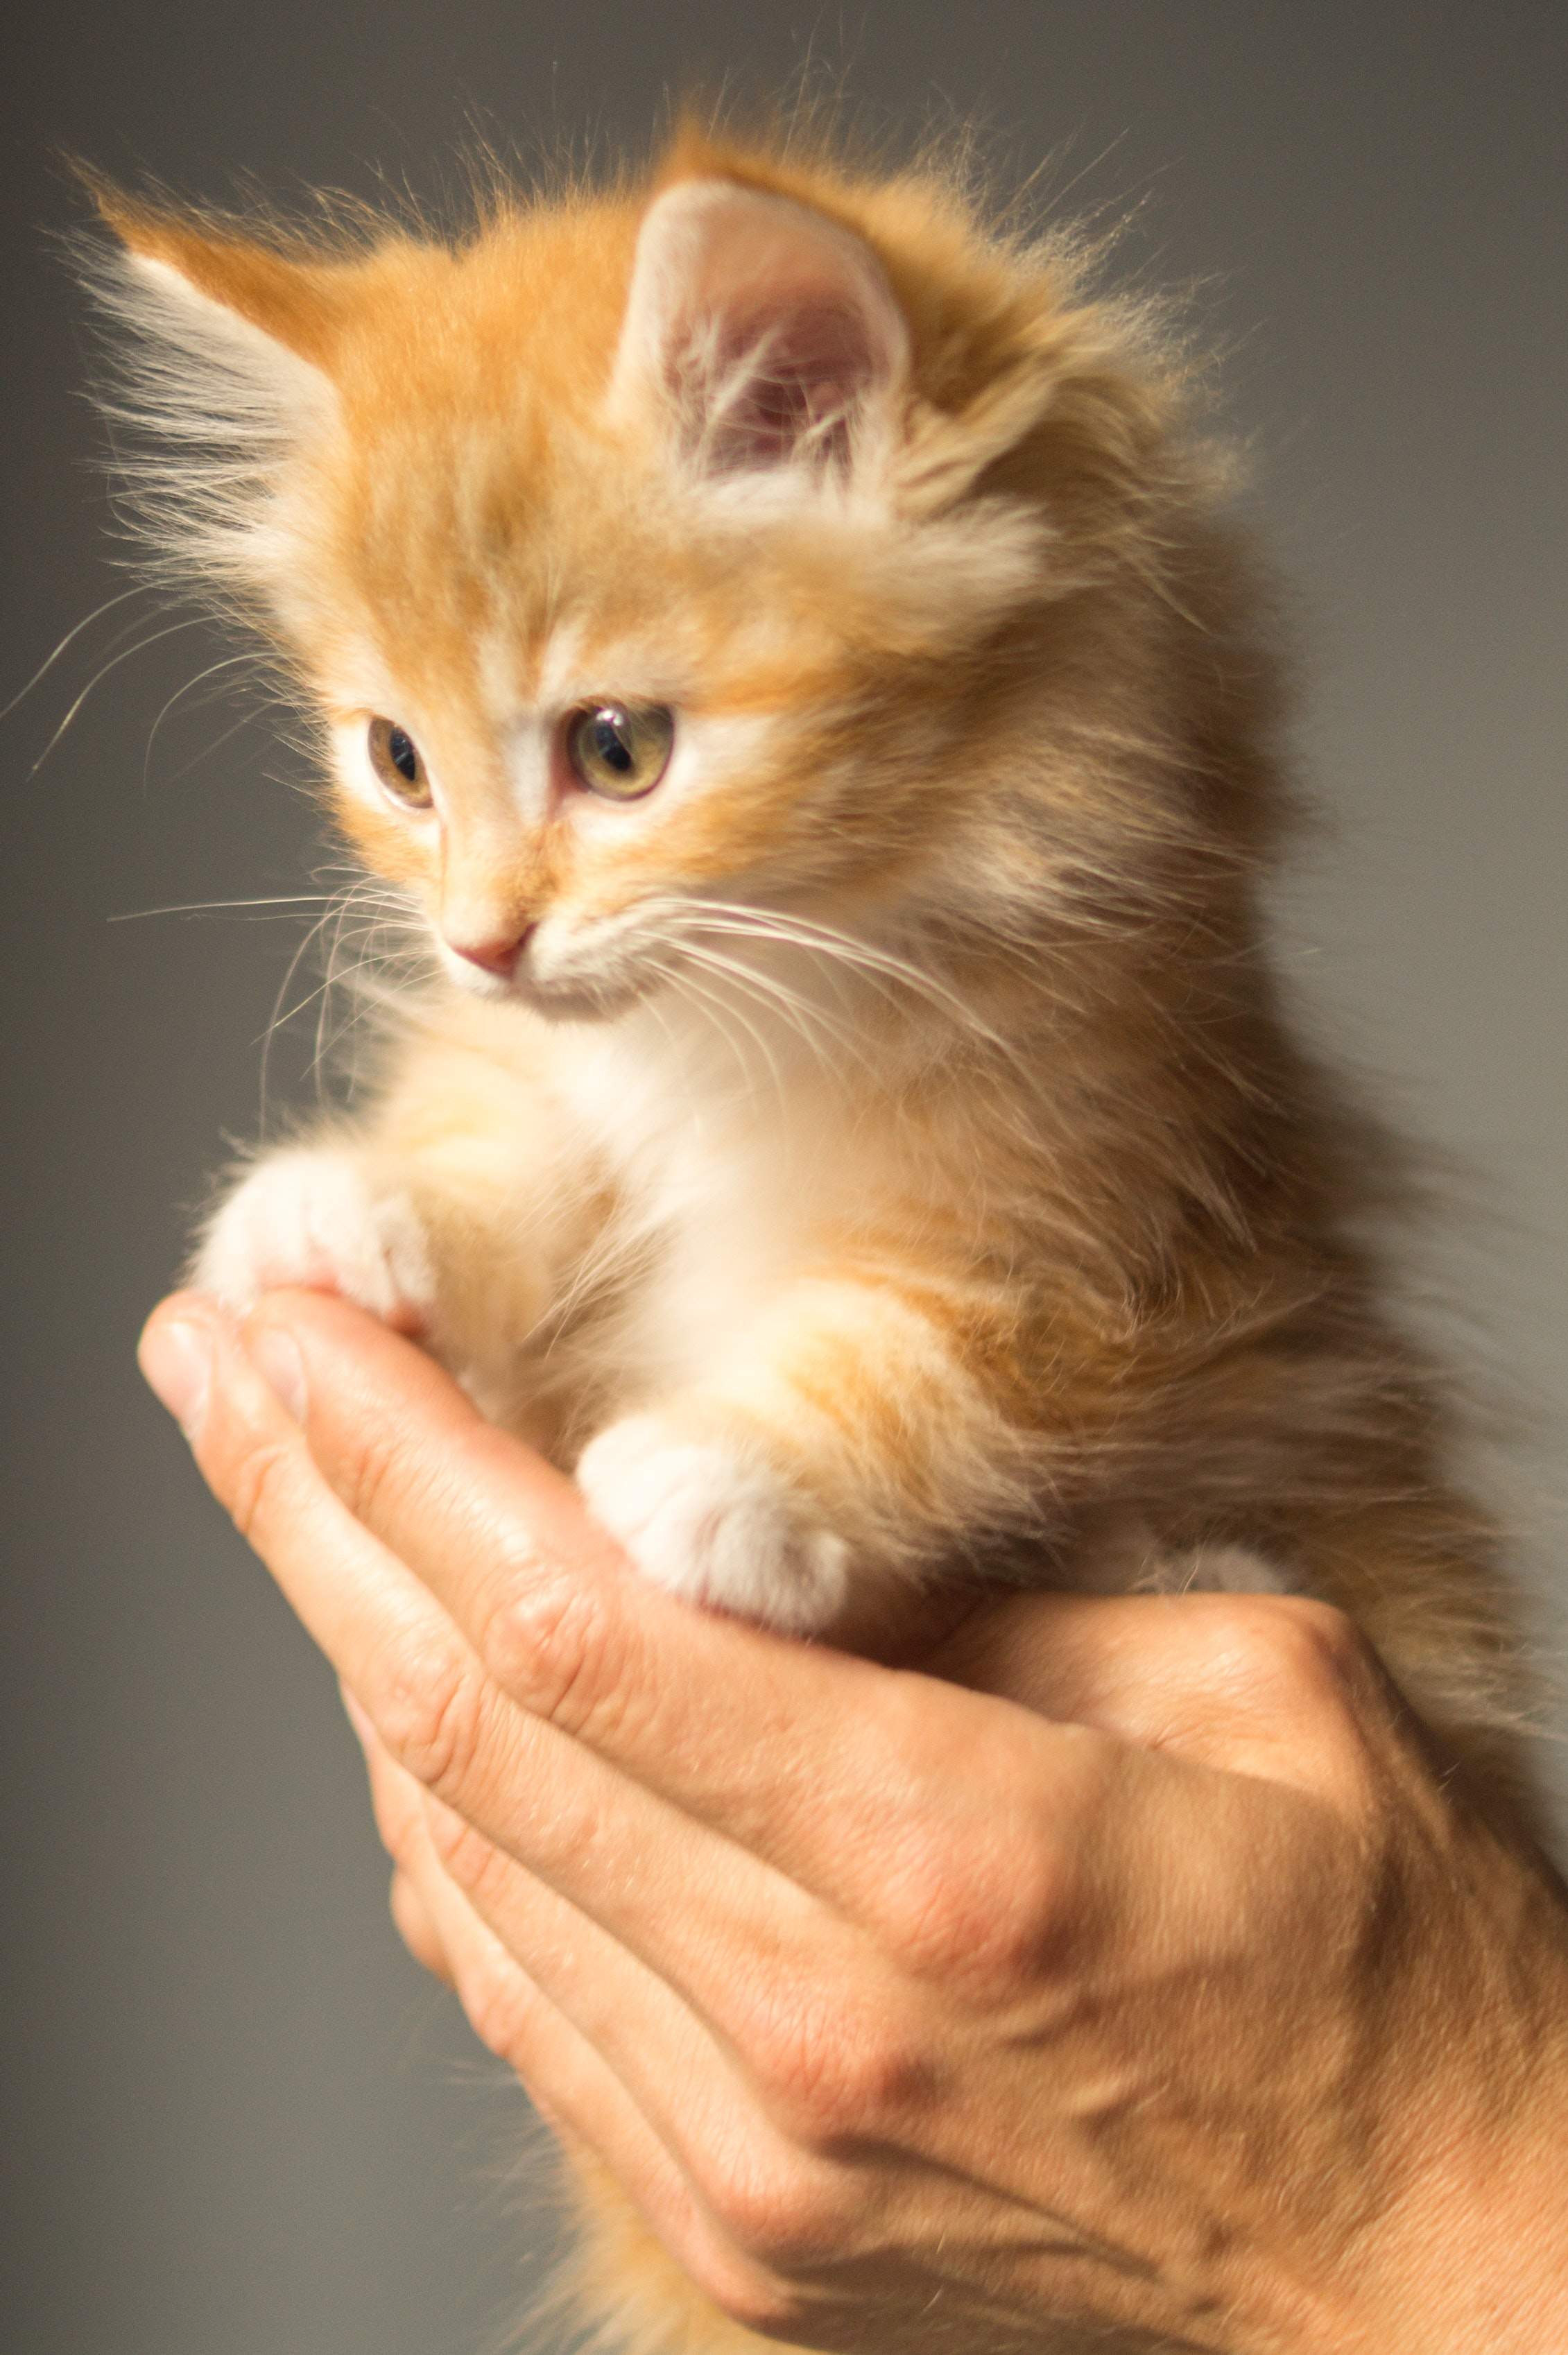
\includegraphics[scale=0.05]{cat.jpg}
%\end{figure}
%%%%%%%%%%%%%%%%%%%%%%%%%%%%%%%%%%%%%%%%%%%%%
%%%%%%%%%%%%%%%%%%%%%%%%%%%%%%%%%%%%%%%%%%%%%
%%%%%%%%%%%%%%%%%%%%%%%%%%%%%%%%%%%%%%%%%%%%%

% End Subsection

\subsection{Requirements}
\label{subsec:requirements}
% Begin Subsection
The DARE design team identified the following requirements to achieve the objectives of this project.
\bigbreak
\subsubsection{Application-Level Requirements}
The DARE engine must:
\begin{itemize}
    \item \textbf{Prediction::} Predict short-term and long-term glucose levels.
    \item \textbf{Factors:} Use historical and current glucose values in conjunction with sleep, diet, exercise and stress to predict future glucose levels.
    \item \textbf{Recommendations:} Generate individualized recommendations for patients.
\end{itemize}

\subsubsection{System-Level Requirements}
The DARE engine must:
\begin{itemize}
    \item \textbf{Modularity:} Be implemented in such a way that each part of the system works independently of other parts in the system.
    \item \textbf{Programming languages:} Be designed using MATLAB, Python, and React Native.
    \item \textbf{Technologies:} Use Docker, Flask, Heroku, and Travis CI.
\end{itemize}

% End Subsection

% End Section

\section{Organization of the Report}
\label{sec:organization_of_the_report}
% Begin Section
This report starts off with a description of DARE's system architecture to illustrate the uniqueness of the model and to show the different components that are involved and how they work together to achieve the project's goal of self-managing diabetes. Then it describes the data generation process that was performed to generate the synthetic glucose and lifestyle data which was used as an input to the prediction engine. 
The mechanism of operation of the glucose prediction engine as well as the goals and outcomes of the model are then discussed in details. Following that, a description of the recommendations engine and how it works to give personalized coaching messages to the patients, based on their predicted glucose levels and the correlation between these glucose values and the lifestyle factors of the patient, can be found. Then the project's ongoing enhancements are discussed as well as the team members' individual contributions. Lastly, a conclusion of the work achieved can be found. 


% End Section

% End Chapter


\chapter{Technical Content}
\label{cha:technical_content}
% Begin Chapter

This chapter contains the technical content related to DARE.

\section{System Architecture}
\label{sec:system_architecture}
% Begin Section
The system architecture of DARE was designed to be modular, scalable, and secure from the ground up. The functions of the system to be provided were broken down into discrete units referred to as modules.

%%%%%%%%%%%%%%%%%%
%%%%%%%%%%%%%%%%%%
%%%%%%%%%%%%%%%%%%
\begin{figure}
\centering
    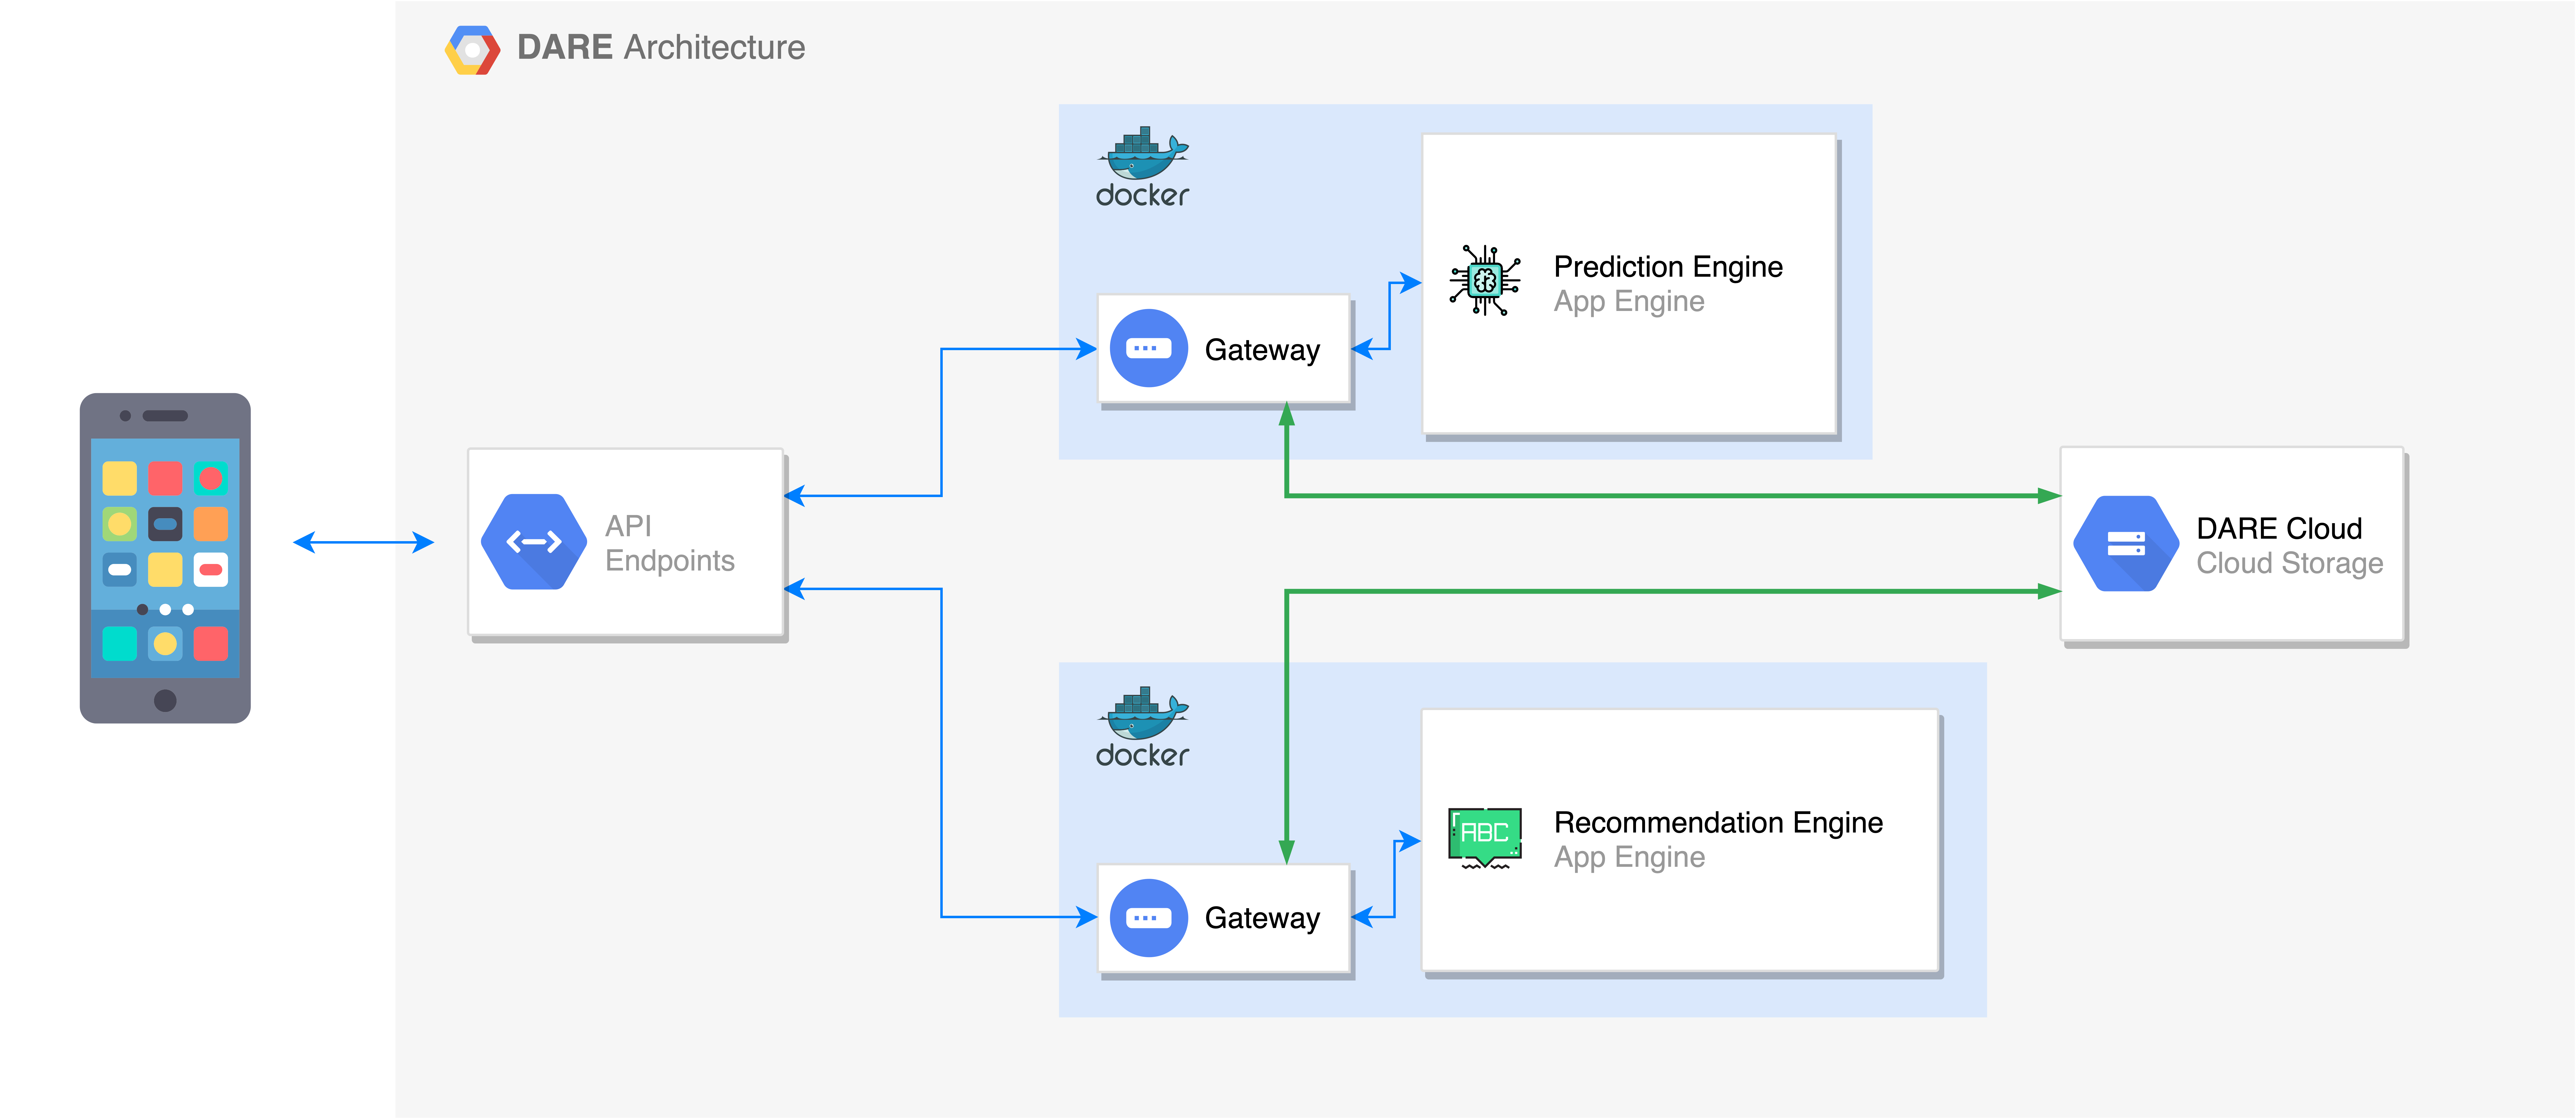
\includegraphics[width=\textwidth]{Figures/Joe/DARE-Architecture.png}
 	\caption{The System Architecture Design}
  	\label{Figure 1}
\end{figure}

\subsection{The DARE Architecture}
The DARE Architecture is composed of a Prediction Engine responsible for making glucose predictions, a Recommendation Engine to generate recommendations based on the available health data, Application Interface to interact with the user and device Application Program Interfaces (API's), and a cloud-based data store for anonymized data storage of datasets.

\subsection{Architectural Design Pattern}
The architecture follows the Service-Oriented Architecture (SOA) design pattern wherein each module serves a distinctive service and every module is unified through a communication protocol established to form the system\cite{17}. The system was primarily broken down into two modules: Prediction Engine and a Recommendation Engine.

\subsection{Enforcing Modularity and Scalability}
Each module was containerized using Docker to ensure encapsulation of functionality furthering the objective of modularity. Containerization also enables scalability through tools like Kubernetes for production-grade container orchestration over cluster-based networks \cite{18}.

Implementation of standardized Representational State Transfer (RESTful) API's for each module transforms them into deployable services that can independently be integrated into 3rd party systems and that cumulatively forms the DARE Architecture.

\subsection{Security and Privacy}
Health data is sensitive and requires careful consideration throughout the data handling process to ensure privacy of the user's data. The DARE Architecture aims to perform partial health data prediction processing on the user's device and sends anonymized data to the architecture modules for further processing, analysis, and persistence.
\bigbreak
The architecture aims to achieve Health Insurance Portability and Accountability Act (HIPAA) compliance through data encryption across information interchange and processing points along with the aforementioned data anonymization \cite{19}.

\bigbreak

% End Section

\section{Application}
\label{sec:engineering_professionalism}
% Begin Section
The mobile application (app) was designed to provide a user-centric experience highlighting key metric useful for the user's health management. The application was built on React Native to provide a native experience for both Android and iOS devices. 

\subsection{Gathering Data}
The app is a crucial gateway to gather the user's health metrics including glucose levels, sleep, exercise, diet, and stress information.
The goal to be achieved through the user experience of this application was to minimize manual data entry and maximize the use of autonomous data sources using smart technologies available to the user. The app aims to gain permissive access to OS health API's (such as Apple Health Kit). Doing so enables data collection from smart wearables and on-device sensors to enable a more accurate form of data input.
Smart voice assistants such Amazon Alexa can also be used with the development of an Alexa skill. A phrase such as "Hey Alexa, tell DARE I took a 7 minute walk" could be channeled as a data input relating to exercise for the Recommendation Engine.

% End Section

\section{Data Generation}
\label{sec:data_generation}

% Begin Section
In order to achieve the objective of this project, a large dataset was required to extract features from and train the prediction and recommendation engines. The dataset required needed to contain glucose levels of diabetic patients over time, as well as lifestyle data such as sleep, exercise, diet and stress. The lifestyle data would normally be acquired automatically using a smart wearable device or through the app by patient input in the ultimate goal of the project. 
In an attempt to obtain such a dataset, several health and research institutions were contacted towards the beginning of the project such as Health Canada, Children's Hospital of Eastern Ontario (CHEO), the National Research Council (NRC), and the Ottawa Hospital Heart Institute. None of these mentioned institutions had such a comprehensive dataset, and it was decided that the data is not readily available. This was the first and biggest challenge faced in this project and in order to overcome it, a data generation algorithm was developed to generate a large dataset of glucose levels under the influence of lifestyle factors. 

\subsection{Patient Profile Creation}
\label{subsec:patient_profile_creation}
% Begin Subsection
In order to develop the data generation algorithm, firstly, an extensive literature review was performed to obtain glucose level datasets under the influence of one of the lifestyle factors mentioned earlier. From this literature review, twelve different profiles were generated, six healthy profiles and six diabetic profiles. For the healthy profiles, profile 1 was obtained from a paper that studied the impact of time of day and sleep on glucose level \cite{7}. Profile 2 was obtained from a paper that studied the effect of a certain type of diet on glucose level \cite{8}. Profiles 3 to 6 were obtained from a paper that studied the effect of different types of exercises on glucose levels \cite{9}.  For the diabetic cases, profile 7 was obtained from a paper that studied glucose level in patients with a regular lifestyle that included general stress, good sleep, and a reasonable diet \cite{10}. Profiles 8 and 9 were obtained from a paper that studied the effect of exercise on diabetic patients \cite{11}.  Profiles 10 and 11 were obtained from a paper that studied the effect of the quality of sleep on glucose level in diabetic patients \cite{12}. For each profile, the obtained data consisted of glucose levels over a 24-hour period in 5-minute interval, and the factor under observation in the literature study. Given that this data comes from literature studies, and the studies include a number of participants to collect the data, the obtained data therefore is the average of the individual participants data. The reason the healthy profiles were generated is due to the availability of data in research studies examining the effect of lifestyle activities on glucose levels in human subjects in comparison to studies on diabetes that include lifestyle factors. A summary of the generated profiles is shown in Table 1.  The obtained glucose level data of the healthy profiles is shown in Figure 1, and that of the diabetic profiles is shown in Figure 2.

\begin{table}[ht!]
	\centering
	\caption{Profiles Generated from a Literature Review on Glucose Levels Change}
	\label{Table 1}
	\begin{tabular}{|c|c|r|}
	\hline
$Healthy (H) or Diabetic (D)$$	 &  $Profile Number$    &   $Lifestyle Factor From Study$ \\
	\hline
	$H$   & 1 & $No Exercise$ \\
	\hline
	$H$   & 2 & $Standing Exercise$ \\
	\hline
	$H$   & 3 & $Walking Exercise$ \\
	\hline
	$H$   & 4 & $Cycling Exercise$ \\
	\hline
	$H$   & 5 & $8 Hours of Sleep$ \\
	\hline
	$H$   & 6 & $Special Diet$ \\
	\hline
	$D$   & 7 & $Good Habits$ \\
	\hline
	$D$   & 8 & $No Exercise$ \\
	\hline
	$D$   & 9 & $Jogging Exercise$ \\
	\hline
	$D$  & 10 & $Stress$ \\
	\hline
	$D$  & 11 & $Enough Sleep$ \\
	\hline
	$D$  & 12 & $Not Enough Sleep$ \\
	\hline
	\end{tabular}
\end{table} 

\begin{center}
\begin{figure}[h!]
	\centering
    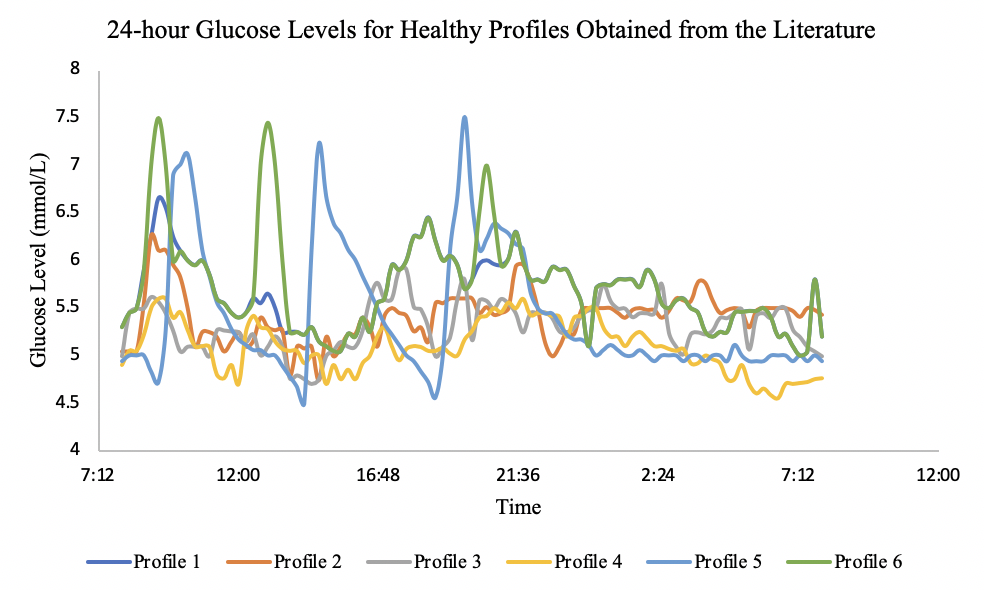
\includegraphics[scale=0.5]{Figures/LEEN/fig1.png}
 	\caption{Glucose Level Data over a 24-hour period as obtained from the Literature Review for Healthy Profiles}
  	\label{Figure 2}
  	
	\centering
    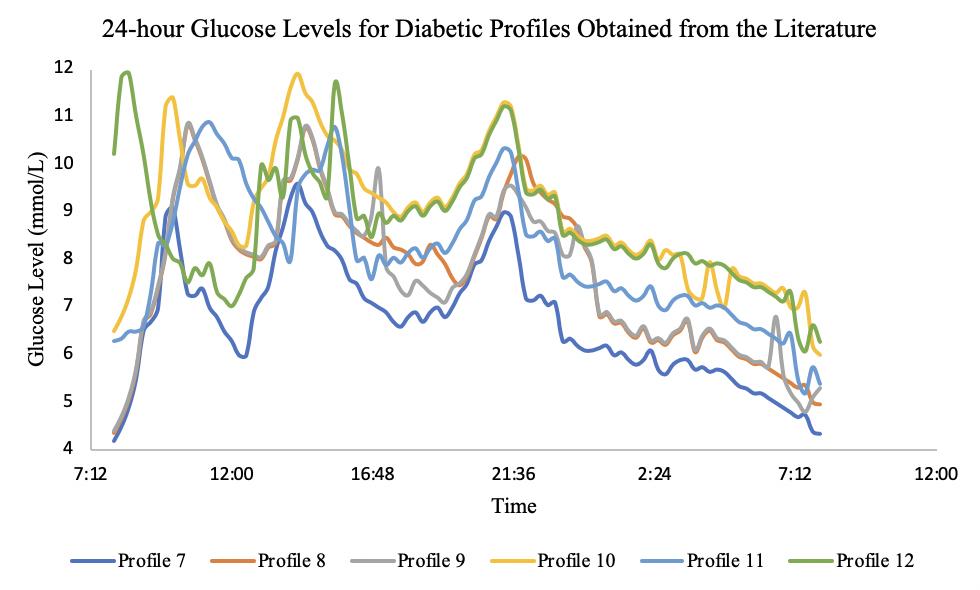
\includegraphics[scale=0.5]{Figures/LEEN/fig2.png}
 	\caption{Glucose Level Data over a 24-hour period as obtained from the Literature Review for Diabetic Profiles}
  	\label{Figure 3}
\end{figure}
\end{center}
% End Subsection

\subsection{Data Generation Algorithm}
\label{data_generation_algorithm}
% Begin SUbsesction
The next step was developing the data generation algorithm to expand the dataset from one day, to 128 days. One of the assumptions made to achieve this goal is that within a profile, the lifestyle factor (or the subject habits) remained consistently similar over the 128 days.
Glucose levels rise significantly after food intake, and therefore there are peaks in the data after participants had their daily meals (breakfast, lunch and dinner). Once the body has metabolized glucose, the glucose levels drop and the baseline glucose level in the bloodstream is observed.
\bigbreak
The data generation algorithm consists of:

\begin{enumerate}
    \item Unit conversion
    \item Peaks detection
    \item Simple random noise addition with a sigma value of 1.8
    \item Horizontal and vertical shifts in the data
    \item Data cleanup 
\end{enumerate}


The algorithm is implemented in MatLab and it utilizes important functions such as peaks detection “findpeaks” and the random function “randi” that selects between different defined cases to apply to the input data to modify it. Additionally, the function that randomly adds white Gaussian noise “normrnd” was also utilized in this algorithm.  
The glucose level data obtained from the literature review was in the unit of mmol/L, in the data algorithm, the data is first converted to the unit of mg/dL.
Then, the peaks in the dataset that occur after food intake are detected and the segments in between the peaks are modified by MatLab by randomly choosing one of five modification cases defined in the algorithm. 
The five defined modification cases include: 

\begin{enumerate}
    \item Shifting the data up and adding white noise 
    \item Shifting the data down and adding white noise 
    \item Shifting the data left and adding white noise
    \item Shifting the data right and adding white noise
    \item Adding white noise without any shifts
\end{enumerate}

With each iteration, the data generation algorithm doubles the amount of input data, and to generate 128 days of data, seven iterations were implemented in the algorithm.

Once the glucose level data was generated, it was observed that some values in the data set were at very low levels that would be considered fatal if they occurred in real life with patients. For this reason, the data was filtered to replace the fatally low glucose values by the minimum acceptable glucose level for healthy and diabetic individuals which was determined to be 80 mg/dL.


% End Subsection

\subsection{Results}
\label{subsec:data_results}
% Begin Subsection
The results from applying the developed data generation algorithm to the 24-hour glucose levels obtained from the literature review were a 128 days of glucose level data for the 12 different profiles. Figure 3 below shows the complete output data for Profile 4, and Figure 4 shows a zoomed in day in February (with the assumption that the first dataset starts on January 1st) for Case 4.

\begin{center}
% Begin Section
\begin{figure}[ht!]
	\centering
    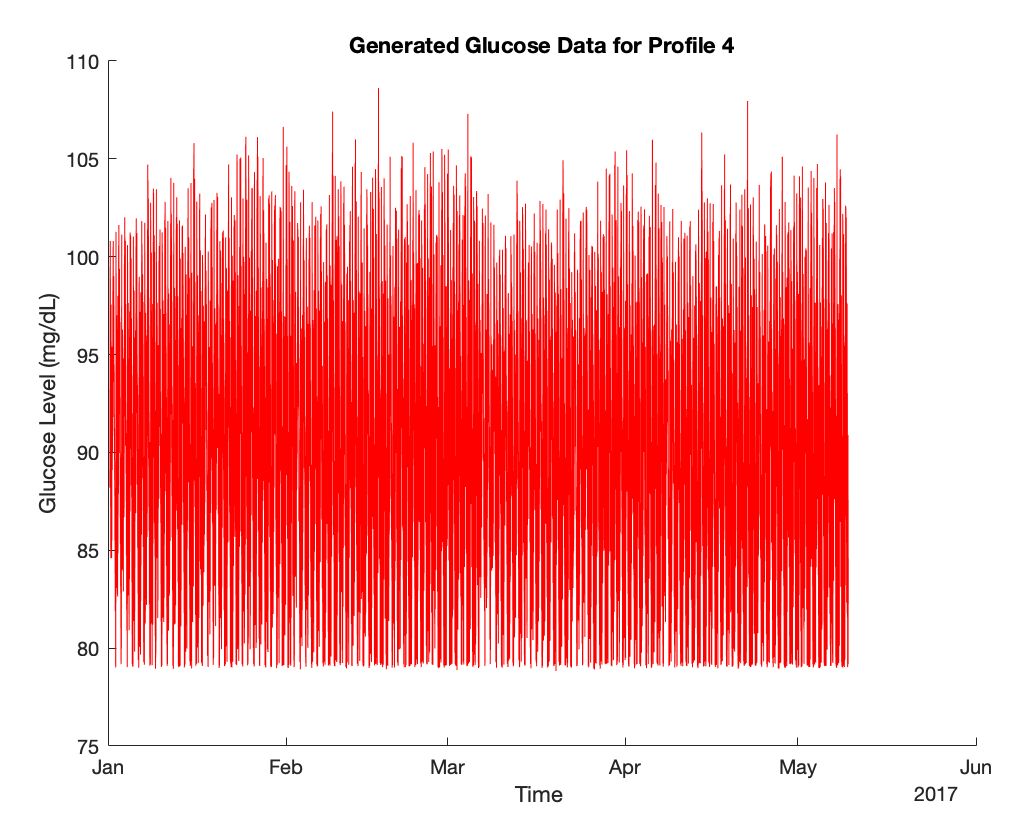
\includegraphics[width=\textwidth]{Figures/LEEN/figure333.png}
 	\caption{Generated Glucose Level Data for Profile 4 over 128 Days}
  	\label{fig-culogo}
\end{figure}
% End Section
% Begin Section
\begin{figure}[ht!]
	\centering
    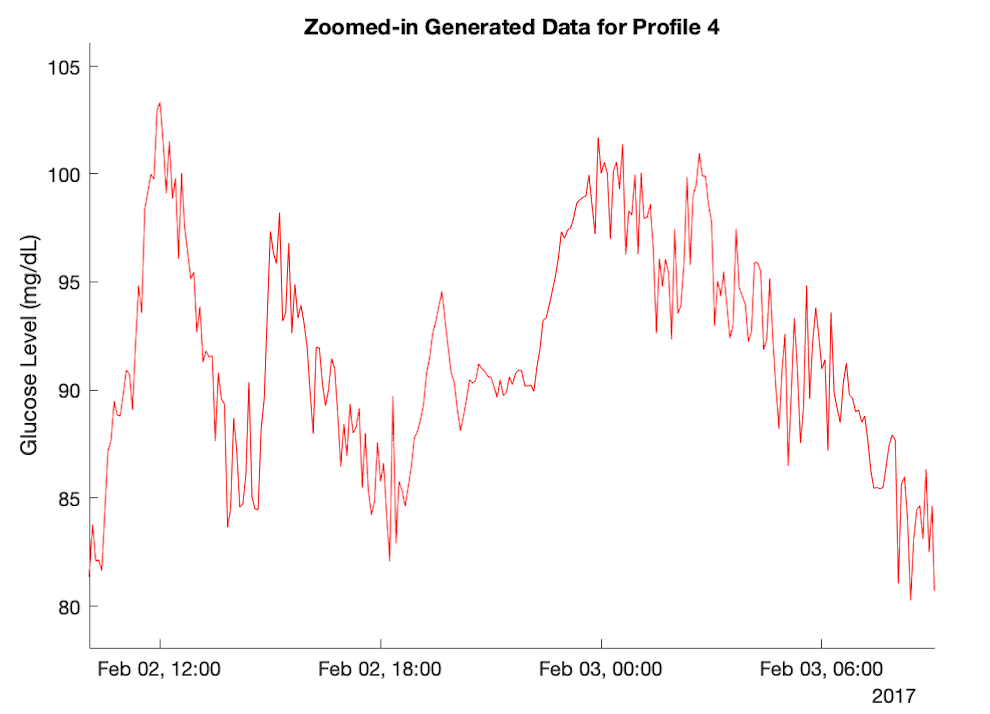
\includegraphics[width=\textwidth]{Figures/LEEN/fig4.png}
 	\caption{Zoomed-in plot of a Day in February from the Generated Data for Profile 4}
  	\label{fig-culogo}
    \end{figure}
% End Section
\end{center}


% End Section
% End Subsection


%%%  PREDICTION ENGINE  %%%

\section{Prediction Engine}
\label{sec:project_management}
% Begin Section Prediction Engine
% Start a new line
% \\Mohamed bluh bluh
% \\* new paragraph format


\bigbreak
The Predictions Engine is responsible for surveying past glucose level data to predict the glucose level for the prescribed time window (such as the next hour, 5 hours, or a day). This predicted glucose value is then channeled to the Recommendations Engine which is responsible for collecting any additional information on factors that impact glucose levels such as diet, stress, sleep, and exercise. Such factors can be retrieved using device health APIs and other smart Internet of Things (IOT) or through smart assistants such as Amazon Alexa. The Recommendations Engine then uses a correlation matrix to identify the most applicable recommendation and sends it to the user through a React Native application.



\subsection{Goals and Requirements}
% Begin subSection Goals and Requirements
The Prediction Engine is responsible for surveying past glucose level data to predict the glucose level for the prescribed time window (such as the next hour, 5 hours, or a day). Thus, there are a number of goals and requirements to consider for the Prediction Engine to achieve. 

\bigbreak

Prediction Engine goals:
\begin{enumerate}
\item Short-Term Prediction
\item Long-Term Prediction
\end{enumerate}

The first goal of the Prediction Engine is to provide glucose level predictions from any where between the next fifteen minutes to the next two hours, known as Short-Term Predictions. Short-Term Predictions are influenced directly by an individual's nutrition's intake in the past half an hour or so. 

The second goal of the Prediction Engine is to provide glucose level predictions for the next day, days, or weeks, known as Long-Term Predictions. Long-Term Predictions are achievable by learning a subject behaviour over long periods in terms of diet, exercise, stress, sleep, insulin intake (if applicable), etc.  

\bigbreak

Prediction Engine considerable requirements:
\begin{enumerate}
\item Computation Complexity
\item Real-Time Processing
\end{enumerate}
	
The system architecture was designed around the Service-Oriented Architecture pattern wherein each unit serves a distinctive function. Containerization enables modularity across the system and scalability using tools like Kubernetes for cluster-based scaling. It also enables independent deployment of each unit and permits third-party entities to integrate a service within their own technologies without requiring dependencies to the rest of the system components.

Therefore, for the Prediction Engine to be applicable in real-life solutions, consideration of computation complexity and real-time processing shall be examined and specified. Furthermore, this examination allows developers to make educated engineering decisions on where to run the Prediction Engine. Such decisions are whether to compute the Prediction Engine under cloud computing, edge computing, combination of edge computing and cloud computing, or even similar mechanism to Search for Extra-Terrestrial Intelligence (SETI) where computation is achieved by utilizing near by peers devices. 

\bigbreak

However, despite the regards to the Prediction Engine requirements examination, the Prediction Engine in this report focuses on the goals of the Prediction Engine; Short-Term Predictions and Long-Term Predictions. The following section, Data Status, discusses the type of expected data the Prediction Engine is suppose to get and what it currently handles.  
% End subSection Goals and Requirements

\subsection{Data Status}
% Begin subSection Data Status
Acquiring full data set is one of the most challenging aspect of this project. This led to significant limitation to the data fed to the Prediction Engine. Figure \ref{data-status} shows an example of the data format that the Prediction Engine received at the time it was being developed. The other expected inputs such as diet, stress, sleep, exercise, insulin intakes, etc, were missing and not available. 

There were other 11 cases similar to the one in Figure \ref{data-status}, glucose level signal over 24 hours, however, they are independent from each others. Thus, predictions are personal-specific.

With that being said, this was the data status the Prediction Engine has had available, and the developers had to move on with what they had. This is part of the unexpected limitations engineers ought to face. The following of the Prediction Engine section elaborates on how it does predictions based only on glucose level signal input for Short-Term Predictions and Long-Term Predictions. 

Furthermore information on how data was handle and generated, refer to the Data Generation Section.  

\begin{center}
\begin{figure}[ht!]
	\centering
    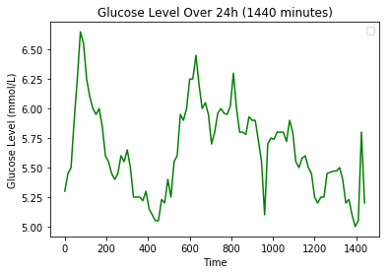
\includegraphics[width=\textwidth]{Figures/mo/data-status.png}
 	\caption{Generated Glucose Level Data for Profile 1 over 24 hours}
  	\label{data-status}
\end{figure}
\end{center}

% End subSection Data Status

\subsection{Prediction Engine Framework Architecture}
% Begin subSection Prediction Engine Framework Architecture
Before moving into the implementation of the Prediction Engine, an abstract design architecture has to be specified to be followed as a framework. 

In general, the Prediction Engine takes in preprocessed filtered data (in this project case, it is only glucose level signal) as input. Then, normalization is applied to the input data, for two reasons; normalization increases consistency, and provokes easier object-to-data mapping resulting in high cohesion and loose coupling. Fair to mention that the normalization affects performance speed as denormalization has to be applied upon output results. Equation \ref{norm} shows how normalization is achieved. 
\begin{equation}
x_{new} = \frac{x-x_{min}}{x_{max}-x_{min}}
\label{norm}
\end{equation}
Feature selection is an important stage in machine learning given that the input data consist of more than one signal. Feature selection is the process of selecting a relevant features of a subset enhancing the performance of a model significantly. However, in this project case, the Prediction Engine predicts glucose level based on previous glucose level signal. The feature selection stage is kept in the framework architecture for future referencing and scalability. 

\pagebreak

The final stages are to use predictive machine learning models to predict glucose level at future time, (t + \ensuremath{\tau}), where t is current time and \ensuremath{\tau} is an interval of a natural number (1, 2, 3 ...). Finally, a delayed error is calculated for model enhancement; the error is delayed as the model has to wait for the actual value of glucose level signal at t + \ensuremath{\tau}. The complete Prediction Engine framework architecture is shown in Figure \ref{arc} below.

\begin{center}
\begin{figure}[ht!]
	\centering
    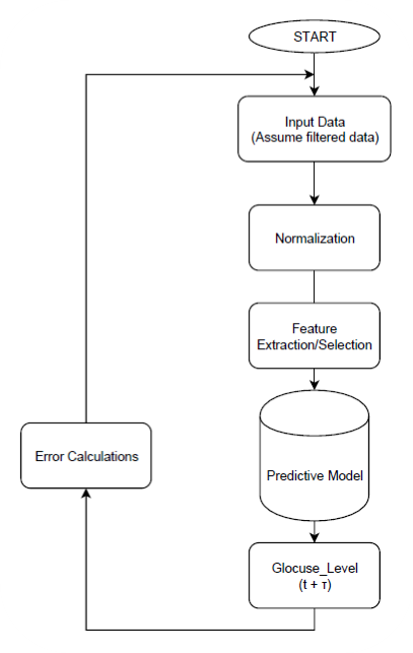
\includegraphics[scale=0.7]{Figures/mo/arc.png}
 	\caption{Prediction Engine Framework Architecture Chart}
  	\label{arc}
\end{figure}
\end{center}
% End subSection Prediction Engine Framework Architecture

\pagebreak

%SHORT TERM PREDICTION
\subsection{Short-Term Prediction: Prototype Model}
% Begin subSection Prototype Model
A prototype model has initially developed to implement short-term predictions. The prototype model is based on a slide window over a glucose level signal (GL), a window size of the slide window, and a predictive interval, \ensuremath{\tau}, which indicates after how much time glucose level to be predicted from current time t. For this prototype model, a 25 minutes window and a 5 minutes predictive interval, \ensuremath{\tau}, were fed to a Simple Linear Regression model (SLR), Equation \ref{lr-eq} . 

\begin{equation}
GL(t) = \beta t + \alpha
\label{lr-eq}
\end{equation}

The input data is fit to SLR to predict GL(t+\ensuremath{\tau}). Figure \ref{slide-fig} visualizes a sample glucose level signal with a slide window and a predictive interval. Figure \ref{lr-fig} shows the results after running the SLR model on a subject. Sharp peeks are presents as the SLR model is linear.     

\begin{center}
\begin{figure}[ht!]
	\centering
    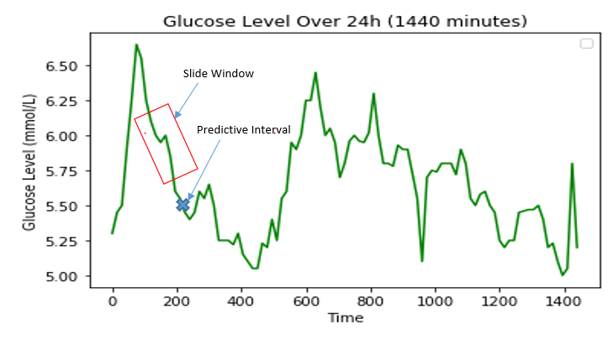
\includegraphics[width=\textwidth]{Figures/mo/slide.png}
 	\caption{Sample glucose level signal with a slide window and a predictive interval}
  	\label{slide-fig}
\end{figure}
\end{center}

\begin{center}
\begin{figure}[ht!]
	\centering
    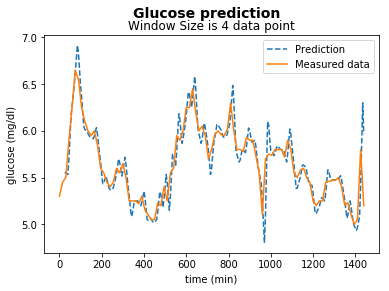
\includegraphics[width=\textwidth]{Figures/mo/lr.png}
 	\caption{SLR model output}
  	\label{lr-fig}
  	
\end{figure}
\end{center}

Regarding error calculations, slide windows predictions are independent from each other, thus, the traditional accuracy error calculations are not suitable in this case. However, the way error is calculated is by squaring the difference between the predictive signal and the actual signal, error difference square (EDS). Figure \ref{lr-eds-fig} shows the effectiveness of the EDS techniques where high magnitude peaks shows where the model performs poorly. To compare the overall performance of a model, the EDS values were added together to give EDS total (EDST).  

\begin{center}
\begin{figure}[ht!]
	\centering
    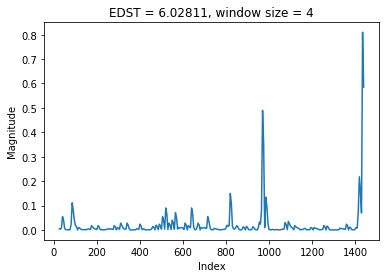
\includegraphics[width=\textwidth]{Figures/mo/lr-eds.png}
 	\caption{Error Difference Square}
  	\label{lr-eds-fig}
\end{figure}
\end{center}

\bigbreak

The approach taken in the prototype model, in terms of a slide window, window size, predictive interval, and error calculations, is continued to be taken for the rest of the short-term prediction models. The ultimate goal for short-term prediction is to have the largest predictive interval, \ensuremath{\tau}, to predict up to the next hour to two hours. The SLR model performs poorly as \ensuremath{\tau} increases. However, in the following sections, more models are explored to give better predictions with increasing \ensuremath{\tau}.
% End subSection Prototype Model

\subsection{Short-Term Prediction: Weighted Linear Regression Model}
% Begin subSection Weighted Linear Regression Model
After implementing the SLR model, Weighted Linear Regression (WLR) model has been implemented where glucose level signal closer to the current time t had more weights, \ensuremath{w_n}, in predicting GL(t+\ensuremath{\tau}), however, it is still linear. Equation \ref{wlr-eq} shows the mathematical representation of the WLR model.

\begin{equation}
\sum_{n=0}^{N}{w_n GL(t)} =\sum_{n=0}^{N}{w_n\beta t + \alpha} 
\label{wlr-eq}
\end{equation}

Similar to LR model, 25 minutes window and a 5 minutes predictive interval, \ensuremath{\tau}, were fed to the WLR model. Then, the input data is fit to the WLR to predict GL(t+\ensuremath{\tau}). Figure \ref{wlr-fig} shows the results after running the WLR model on a subject. Sharp peeks are presents as the WLR model is still linear, however, its performance is slightly better than the SLR model as it has lower EDST value. 


\begin{center}
\begin{figure}[ht!]
	\centering
    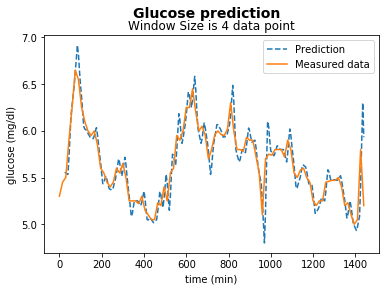
\includegraphics[width=\textwidth]{Figures/mo/wlr.png}
 	\caption{WLR model output}
  	\label{wlr-fig}
\end{figure}
\end{center}
% End subSection Weighted Linear Regression Model

\subsection{Short-Term Prediction: Support Vector Regression Model}
% Begin subSection Support Vector Regression Model
A more sophisticated non-linear model needed to be implemented to have a better performance. A popular machine learning regression model that fits the aforementioned criteria is Support Vector Regression (SVR) model. 

Essentially, SVR is a linear model where regression is based on two vectors surrounding data of interests. In opposition to SLR where a vector passes through the of data of interests, SVR passes two vectors surrounding all data of interests. In practice, SVR has better performance than SLR. Nevertheless so far, SVR is a linear model.

Furthermore, SVR were further improved to enhance non-linear data. Thus, there are two modes of SVR; linear mode and kernel mode. Linear mode is not suitable for non-linear curves. To resolve this matter, the kernel mode is applied where data are transformed into a higher dimensional space using kernel functions, thus, linear separation is feasible.

As expected, SVR has had significant better predictions than SLR and WLR for larger window sizes and predictive intervals. Figure \ref{svr-fig} shows the results of running SVR with a window size of 45 minutes and a 25 minutes predictive interval.

\begin{center}
\begin{figure}[ht!]
	\centering
    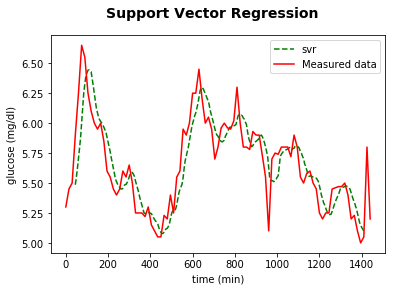
\includegraphics[width=\textwidth]{Figures/mo/svr.png}
 	\caption{SVR model output}
  	\label{svr-fig}
\end{figure}
\end{center}
% End subSection Support Vector Regression Model

\subsection{Short-Term Prediction: Random Forest Regression Model}
% Begin subSection Random Forest Regression Model
Random Forest Regression (RFR) model operates by constructing multiple decision trees at training time to output a mean prediction regression model.

RFR model outperformed SVR for the same window sizes and predictive intervals. Figure \ref{rfr-fig} shows the results of running RFR with a window size of 45 minutes and a 25 minutes predictive interval.


\begin{center}
\begin{figure}[ht!]
	\centering
    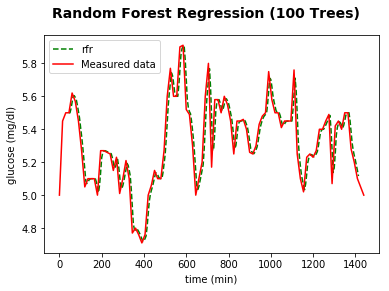
\includegraphics[width=\textwidth]{Figures/mo/rfr.png}
 	\caption{RFR model output}
  	\label{rfr-fig}
\end{figure}
\end{center}
% End subSection Random Forest Regression Model

\pagebreak 

\subsection{Short-Term Prediction: Model Comparison}
% Begin subSection Model Comparison
As all the short-term prediction models (SLR, WLR, SVR, RDR) were discussed separately, Figure \ref{cmp-fig} shows results for running different window sizes and predictive intervals. RFR had the best overall performance regardless of the number of trees used. It has the lowest EDST value of all of the other models. 

The max predictive interval that was testes is 30 minutes in that table, however, 45 minutes were presented in SVR and RFR section. As mentioned before, although the goal is to have the predictive interval up to 2 hours, all the models were not tested beyond 45 minutes. The reason was related to the discovery of time-series analysis and its effective approach. 

The next section elaborates more on time-series analysis approach and its effectiveness on short-term and long-term predictions.

\begin{center}
\begin{figure}[ht!]
	\centering
    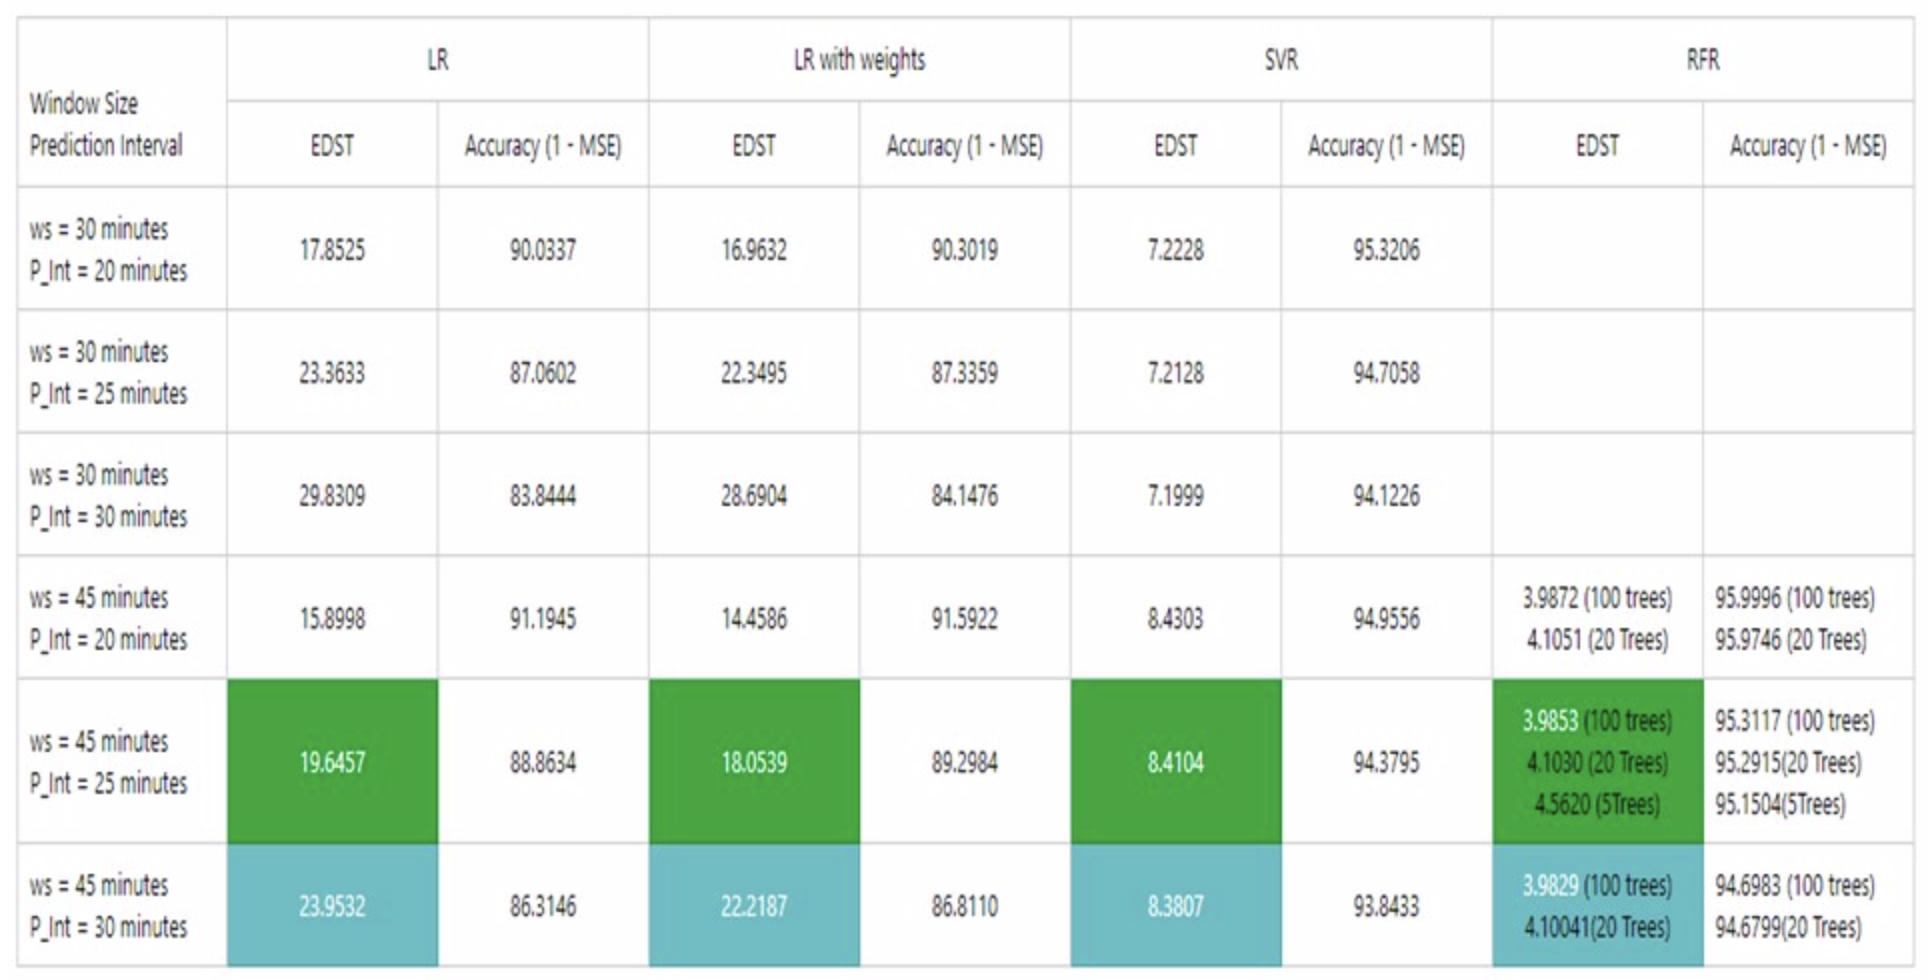
\includegraphics[width=\textwidth]{Figures/mo/cmp-models.png}
 	\caption{Short-Term Predictions: Model Comparison}
  	\label{cmp-fig}
\end{figure}
\end{center}
% End subSection Model Comparison

\subsection{Long-Term Prediction: Time-Series Analysis}
% Begin subSection Time-Series Analysis

The second goal of the Prediction Engine is to provide glucose level predictions for the next day, days, or weeks, known as Long-Term Predictions. The parameters to be fed in the Prediction Engine for Long-Term Predictions were expected to be diet, exercise, stress, sleep, insulin intake (if applicable), etc. However, as discussed in the Data Status section, only glucose level signal was actually input to the Prediction Engine. 
Please note this section provides a paradigm on how to implement Long-Term Predictions using time-series analysis with neural networks. The implementation has not been completely done due to time limitation. 

An intelligent way to achieve predictions in this scenario is to learn the behaviour of the signal and predict based on that \cite{time-series-paper}. In other words, the signal itself is the input for the Prediction Engine independent from time (no time vector is input). This is also known as time-series analysis, elaborated more in Figure \ref{time-series} and Equation \ref{time-series-eq}. 

\begin{equation}
GL(t)_i = \beta GL(t)_{i-1} + \alpha
\label{time-series-eq}
\end{equation}

\begin{center}
\begin{figure}[ht!]
	\centering
    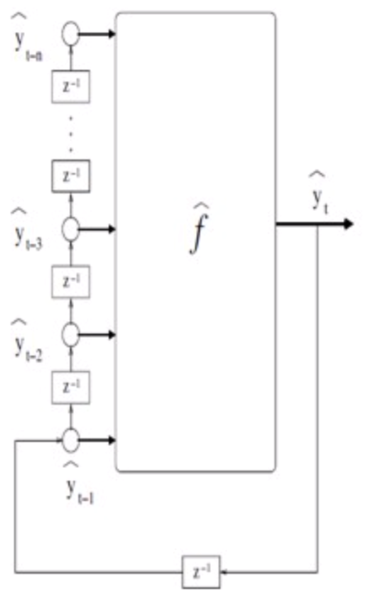
\includegraphics[scale = 0.6]{Figures/mo/time-series.png}
 	\caption{Time-Series: iterated prediction. The approximator f returns the prediction of the value of the time series at time t+1 by iterating the predictions obtained in the previous steps. (the rectangular box contain z represents a unit delay operator)}
  	\label{time-series}
\end{figure}
\end{center}

Good models to utilize in order to achieve Long-Term Prediction are time-based neural network models such: 

\begin{enumerate}
\item Long-Short Term Memory LSTM
\item Feed-Forward Neural Network FFNN
\item Recurrent Neural Network RNN
\end{enumerate}

For neural network models, X-train and Y-train have to constructed based on time-series analysis mentioned above. Figure \ref{time-series-app} shows X-train and Y-train construction. 

The first row of X-train is the all previous glucose levels and the first row of Y-train \ensuremath{G_i} is the glucose level value at current time t.

\begin{enumerate}
\item Iteration 1:  the first X-train and Y-train row are input to a neural network model to predict the next row of Y-tain \ensuremath{G_{i+1}}. 

\item Iteration 2: \ensuremath{G_i} is inserted to the end of the second X-train row shifting the vector to the left. Then, the first and second row of X-train and Y-train are input to the neural network model to predict the following glucose level \ensuremath{G_{i+2}}.
\end{enumerate}

The following iterations are repeated identical to iteration 2 above. In each iteration, a new predicted value is inserted to the end of the X-train vector. The model keeps predicting and iterating until all the values in the X-train vector are all predicted values. The longer the X-train vector in iteration one, the longer predictions the model would generate. 

This methodology trains neural network models to learn the behaviour of the signal based on time-series analysis. Nevertheless, X-train and Y-train could also be utilized in training other regression models such as SVR and RFR, to generate Long-Term Predictions and expected to match neural network performance.



\begin{center}
\begin{figure}[ht!]
	\centering
    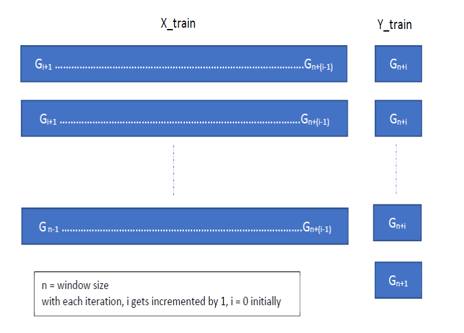
\includegraphics[width = \textwidth]{Figures/mo/time-series-app.png}
 	\caption{Prediction Engine: applying Time-Series}
  	\label{time-series-app}
\end{figure}
\end{center}

Once again, please note this section provides a paradigm on how to implement Long-Term Predictions using time-series analysis with neural networks. The implementation has not been completely done due to time limitation.
% End subSection Time-Series Analysis

\subsection{Prediction Engine Integration}
% Begin subSection Prediction Engine Integration

The Prediction Engine shall not be limited to the application of a model discussed above. In other words, different models could be integrated together in order to get the best end results. The integration is not internally among models but rather externally to maintain modularity within the engine. For example, with regards to the outperforming models, the end results of glucose level predictions could be integrated using different methodologies such as arithmetic mean, geometric mean, or mid-range in a range of acceptable glucose level values.

% Expert System – Model Aggregation
% Processing Requirements and Speed
% Optimization Decisions

% End subSection Prediction Engine Integration


% End Section Prediction Engine





\section{Recommendation Engine}
\label{sec:recommendation_engine}
% Begin Section
One of the main objectives of DARE was to provide meaningful, individualized recommendations to T2DM patients to manage their diabetes. Ideally, users are able to enter all of the required data into an app which uses the DARE engine. This allows the DARE engine to provide highly individualized recommendations that would get better with time. However, this may not be the case and as such, the design team made decisions to allow the Recommendation Engine (RE) to provide the most accurate recommendations regardless of how much data was available. Consequently, the following architecture for the RE was developed.

\subsection{Recommendation Engine Architecture}
\label{subsec:re_architecture}
% Begin subsection
The RE consists of five main components (Figure \ref{fig:re}):

\begin{enumerate}
    \item Inputs
    \item Weighted-factor analysis module
    \item Single-factor analysis module
    \item Recommendation generator
    \item Output
\end{enumerate}

\begin{figure}[ht!]
    \centering
    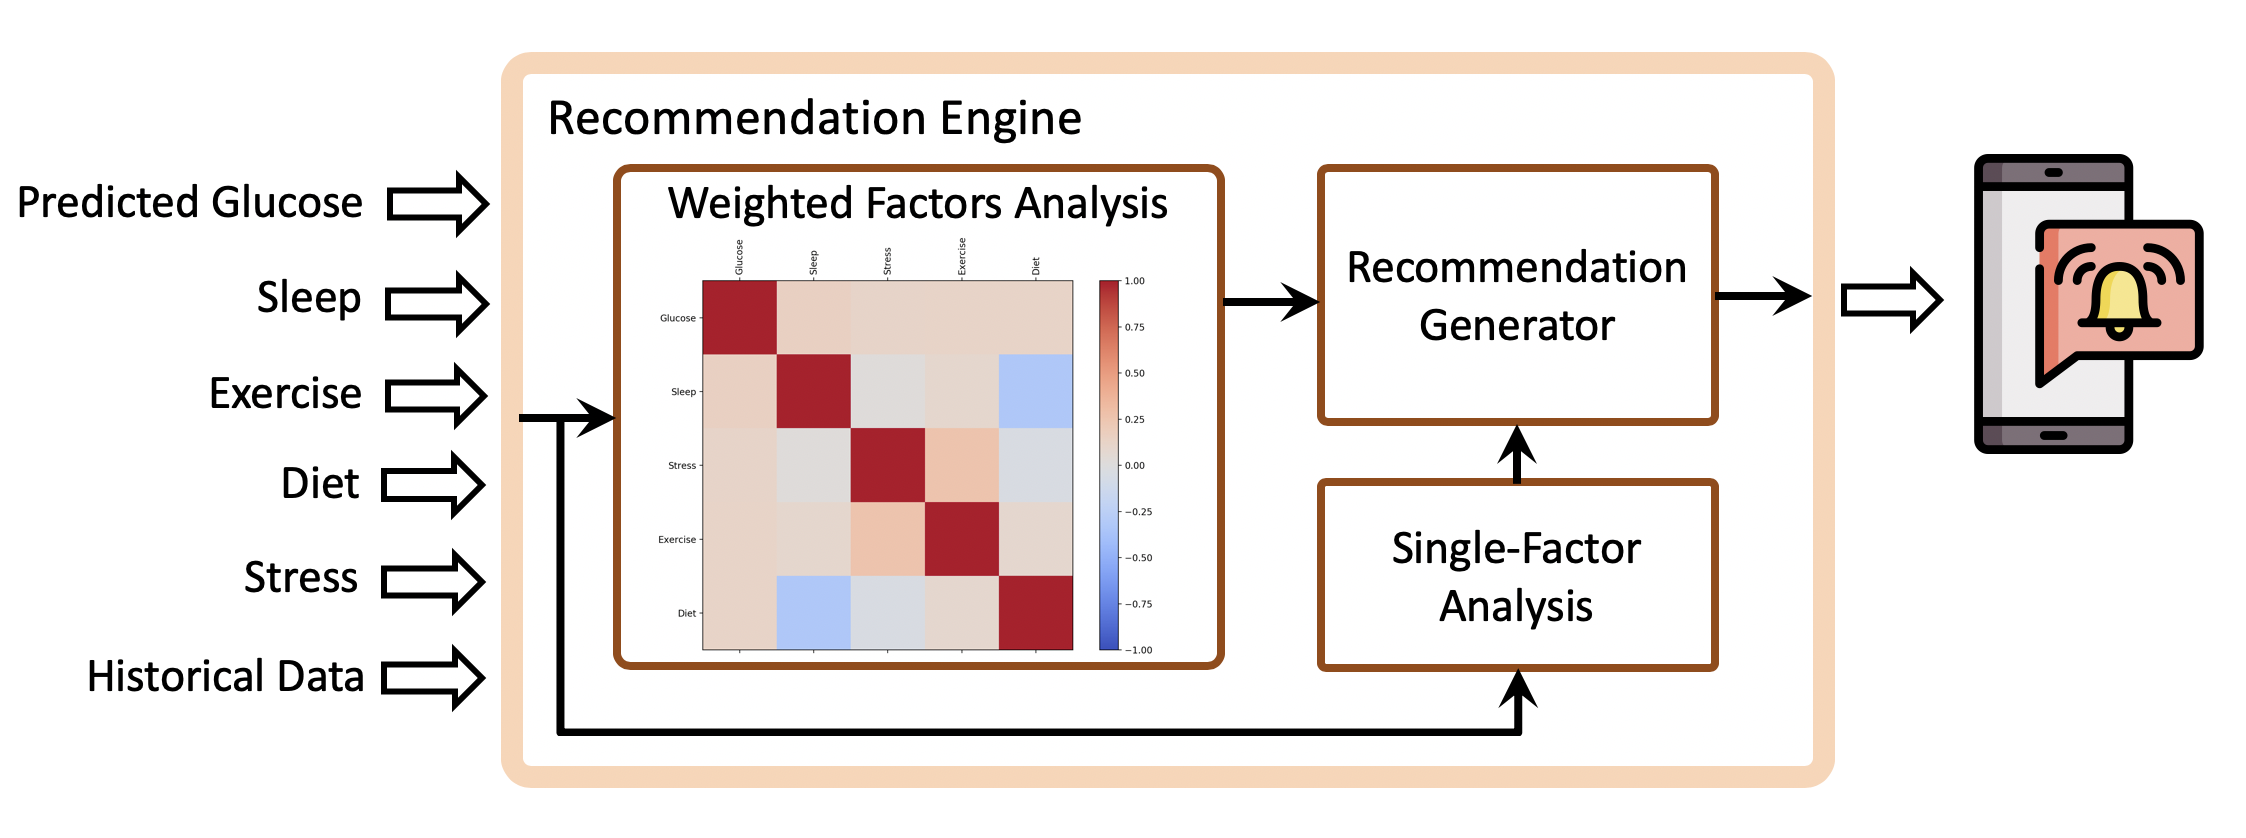
\includegraphics[width=\textwidth]{Figures/pooria/re.png}
    \caption{Recommendation Engine's Modular Architecture}
    \label{fig:re}
\end{figure}

This architecture has the advantage of leveraging full modularity meaning that each component inside the engine can work independently of other. This allows for not only a cleaner design but also one which is scalable and can easily be customized based on the specific application that is being used. For instance, there many algorithms in order to calculate the correlation between factors. Having a modular design allows the developers to modify the Weighted-Factor Analysis module to use their desired algorithm without having to change any other part in the engine.

Furthermore, the RE architecture generates recommendations based on the availability of data. This flexibility has been taken into account to ensure the RE can continue to provide appropriate and accurate recommendations regardless of which factors are available. This flexibility is achieved by creating two separate modules one of which deals with cases where only glucose is available and one where other factors are available as well.

% End subsection

\subsection{Single-Factor Analysis}
\label{subsec:single_factor_analysis}
% Begin subsection
This module was designed to handle cases where only predicted glucose data is available. Essentially, once the RE detect that only glucose data is present, the Weighted-Factor Analysis module is bypassed, and the recommendations generated are purely based on glucose values. In this case, a minimum and maximum acceptable glucose level is selected from a look up table file based on the time of the day and the patient is given recommendation based on whether they meet the acceptable levels of glucose. The patient is also prompted with a message encouraging them to input more data to receive more individualized recommendations.
% End subsection

\subsection{Weighted-Factor Analysis}
\label{subsec:weighted_factor_analysis}
% Begin subsection
This module was designed to provide accurate predictions based on the presence historical data on the five factors of glucose, exercise, sleep, diet, and stress. This module calculates the correlation between the latter four factors (the ones available) and glucose, ranking them based on the extent to which they affect glucose levels. After the ranking has been done through a correlation method in Python, the recommendations are provided to the patient based on the highest ranked factor. The level of sophistication added to the RE by this module ensures that the recommendations given are based on their predicted glucose levels as well as the historical data of each patient creating a more individualized and accurate recommendation.

In this implementation of the Weighted-Factor Analysis module, the “corr()” method from the “pandas” package was used, allowing for an easy and flexible analysis of the correlations. Furthermore, while the corr() method allow for the choice between “Pearson’s R”, “Kendall’s Tau” and “Spearman Rank Correlation”, the correlation method selected in this implementation was the “Spearman Rank Correlation”  as this is the only method which does not assume the data to be normally distributed. Furthermore, Spearman rank correlation is a good fit for monotonic data which have a predictable behaviour (monotonic) as well as ordinal data \cite{13},\cite{14}. For instance, from literature has shown that higher stress levels can raise baseline glucose levels \cite{15}. In this case, the relationship is both monotonic and stress is an ordinal variable (subjectively ranked on a 1-5 scale by the patient). As a result of this, the Spearman rank correlation was a good fit for this application.

Lastly, the advantage of this modular approach is that developers can easily replace the correlation algorithm with any other ones they would like without having to majorly change the code or having to make modification to other parts of the RE.

% End subsection

% End Section

\subsection{Recommendation Generation Algorithm}
\label{subsec:recommendation_generation_algorithm}
% Begin subsection

The recommendation algorithm was designed as a basis to the RE to consider cases where the predicted GL would be normal or outside of the normal range. The possible cases or routes to a final recommendation can be summarized as follows:

\subsubsection{Case 1: Normal GL and normal available factors}
In this case, the RE produces a message informing the patient that their GL is within range followed by an encouraging message to keep up their good habits. An example recommendation for this case is “Great! Your glucose is within range. Keep monitoring your glucose levels and continue practicing your healthy habits.”

\subsubsection{Case 2: Normal GL but poor factors detected}
In this case, the patient may have a GL within the normal range, but the algorithm detects an unhealthy habit pertaining the four factors of exercise, sleep, diet and stress. Although the GL is currently predicted to be within range, the continued practice of the poor habits may result in long-term negative impact on the patient’s GL. As an example, a patient may have a GL value within range, but they may have slept for only 5 hours the night before. The algorithm produced a recommendation informing the user of their normal GL but that getting enough sleep can help them maintain such normal levels in the long run. As another example, a patient who has a normal GL but high levels of stress will receive a recommendation which acknowledges the normal glucose level while also being informed of possible options, such as deep breathing, to lower their stress.

\subsubsection{Case 3: GL is outside of normal range and other factors are unavailable}
In this case, the recommendation algorithm provides a prompt to the user to add more information on the unavailable factors. If the user does not provide additional information, the recommendation engine will perform a single-factor analysis (See section 2.5.2) to provide a generic recommendation. As an example, if the GL is below the normal range, the recommendation provided will encourage the patient to snack to raise their GL. On the other hand, if the GL are higher than the maximum normal value, the recommendation will encourage the patients to engage in activities such as exercise or stress management to lower their GL.

\subsubsection{Case 4: GL is outside of normal range and other factor are available}
In this case, in addition to predicted GL, other factors are available as well allowing the RE to perform a weighted-factor analysis (See section 2.5.3) to provide specific and individualized recommendations. As an example, the correlation algorithm determines that sleep has the most negative impact on this particular patient and given the GL of the patient is outside of the normal range, the patient will receive a recommendation pertaining to how sleep can help them manage their GL.


\begin{figure}[h!]
    \centering
    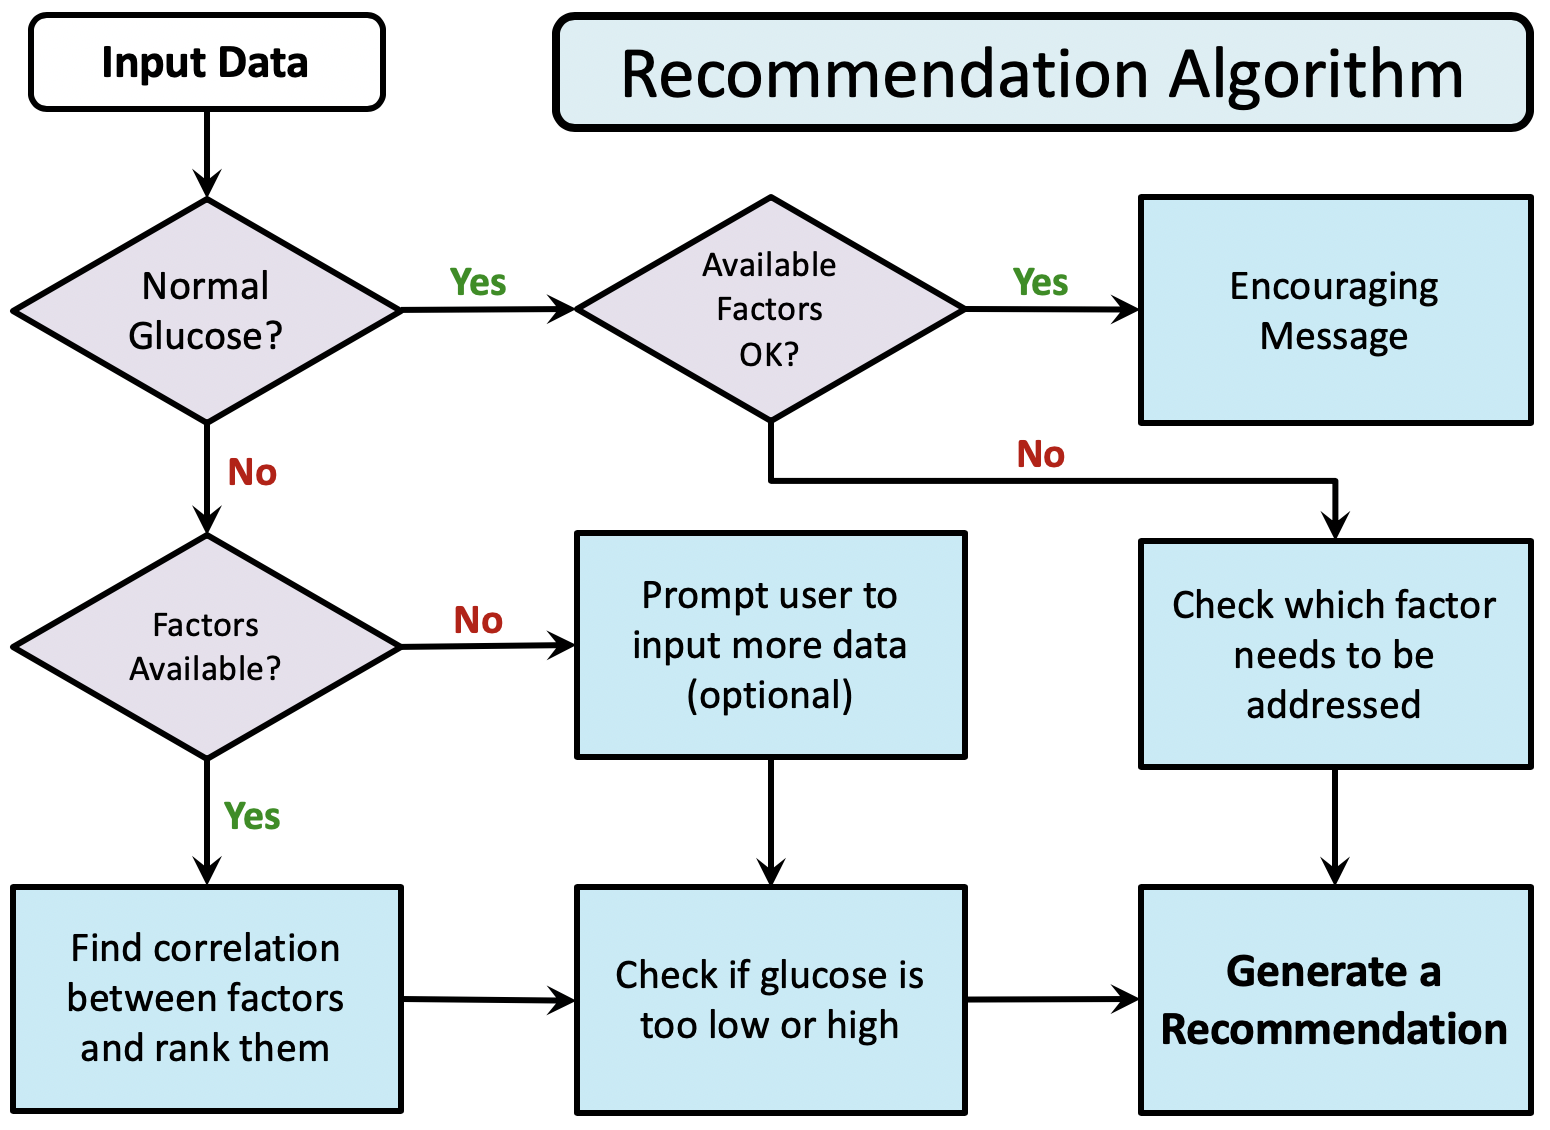
\includegraphics[scale=0.4]{Figures/pooria/re_alg.png}
    \caption{Recommendation Generation Algorithm}
      \label{fig:re_alg}
\end{figure}
% End subsection

% End Section

\chapter{Ongoing Enhancements}
\label{sec:ongoing_enhancements}
% Begin Section
The DARE Architecture was built to take the next step in diabetic-based assistive health technologies for patients to effectively manage their glucose levels and receive comprehensive recommendations thanks to ever personal smart technologies.
The architecture can be further enhanced to provide more robust set of nuanced predictions and recommendations with refinements in neural network models and improved correlation datasets. 
Correlated datasets can be validated by active application users to collect a open-source version of diabetic data with correlations between glucose levels, sleep, diet, exercise, and stress. This dataset can be used in the development of a richer neural network and opened up to the research community.
An improved Recommendation Engine model can be trained to enhance parallel correlations among multiple data sources and account for the psychological effect caused by the recommendations generated to the user.
Support for increased native OS-based health API's and smart IOT devices can be harnessed to improve input accuracy for data sources to the architecture.

% End Section

\chapter{Conclusion}
\label{sec:conclusion}
% Begin Section
The project aimed to tackle the challenge of assisting diabetic patients in effectively managing their glucose levels through sporadic context-driven recommendations.

The DARE Architecture was developed to cater to the afformentioned objective through the coalescing of a Prediction Engine and Recommendation Engine driven by consolidated user health data.

The architecture, inspired by the Service-oriented Architecture design pattern, was built from the ground-up to ensure scalable and modular deployments through containerization. 

The client-side application minimized input data inaccuracies through increased focus on autonomous data collection from available IOTs and smart technologies predicating user permissions. 

Synthetic data was developed to train mathematical regression models for glucose level predictions based on past trends. Variable input sources for the Recommendation Engine ensures the generation of timely context-driven recommendations to assist in glucose level management.



% BEGIN COMMENT
\begin{comment}
        Briefly summarize the problem, the solution, and your accomplishments towards the solution. (Remember,
        you want to be very clear about the answers to the BIG 3 questions!) Be sure to point out any features that
        might make your solution more desirable than other existing solutions to similar problems. 
        
        Make suggestions about how the project might be extended or modified to solve bigger or related problems.
        You do not have to give many details here, but a brief description will help the reader follow your
        suggestion.
        
        During a project (and particularly near the end), it is not unusual for new alternative solutions to be
        discovered. Often, the project is committed to a particular solution and too much work would be involved
        to incorporate the new solution. If this happens, you might want to describe the new solution and
        recommend that the new solution might be preferable to the one you implemented. 
\end{comment}
% END COMMENT

% End Section

\chapter{Individual Contributions}
\label{sec:individual_contributions}
% Begin Section
This section lists the individual contributions towards the various project deliverables
% End Section

\section{Project Contributions}
\label{sec:project_contributions}
% Begin SubSection

\begin{tabular}[t]{l@{\hspace*{2cm}}l}
	Data Generation: & Pooria, Leen, Lama \\
    Prediction Engine: & Mohamed \\
	Recommendation Engine: & Pooria \\
	Application: & Joe \\
	System Architecture, Integration, and Deployment: & Joe \\
\end{tabular}

% End SubSection

\section{Report Contributions}
\label{sec:report_contributions}
% Begin SubSection
\begin{tabular}[t]{l@{\hspace*{2cm}}l}
	Abstract: & Lama \\
	Introduction: & Lama, Pooria \\
	Acknowledgements: & Pooria \\
	List of Abbreviations: & Pooria \\
	System Architecture: & Joe \\
	Application: & Leen, Lama \\
	Data Generation: & Leen, Lama\\
	Prediction Engine: & Mohamed \\
	Recommendation Engine: & Pooria \\
	Ongoing Enhancements: & Joe \\
	Conclusion: & Joe \\
\end{tabular}
% End SubSection

% References
\renewcommand{\bibname}{References}
\begin{thebibliography}{AAA}	
\bibitem {1} D. Of and D. Mellitus, “Diagnosis and classification of diabetes mellitus,” Diabetes Care, vol. 37, no. SUPPL.1, pp. 81–90, 2014. 

	      
\bibitem{2} “Diabetes,” Heart and Stroke Foundation of Canada. [Online]. Available: https://www.heartandstroke.ca/heart/risk-and-prevention/condition-risk-factors/diabetes.

\bibitem {3} H. Wu, S. Yang, Z. Huang, J. He, and X. Wang, “Type 2 diabetes mellitus prediction model based on data mining,” Informatics Med. Unlocked, vol. 10, no. December 2017, pp. 100–107, 2018.

\bibitem{4} “The Best in Diabetes Management,” One Drop. [Online]. Available: https://onedrop.today/.


\bibitem{5} “Award-Winning Diabetes Tools,” Glucose Buddy. [Online]. Available: https://www.glucosebuddy.com/.

%%%% DO NOT CHANGE THE NUMBERS INSIDE CURLY BRACKETS PLEASE
\bibitem {6} D. I. C. Production Assistant, “BlueStar Diabetes,” Diabetes In Control. A free weekly diabetes newsletter for Medical Professionals..., 19-Aug-2017. [Online]. Available: http://www.diabetesincontrol.com/bluestar-diabetes-2/. 

%%%% DO NOT CHANGE THE NUMBERS INSIDE CURLY BRACKETS PLEASE
\bibitem{17}
“Service-oriented architecture (SOA),” IBM Knowledge Center. [Online]. Available: https://www.ibm.com/support/knowledgecenter/en/SSMQ79$_$9.5.1/com.ibm.egl .pg.doc/topics/pegl$_$serv$_$overview.html. [Accessed: 01-Apr-2019].

%%%% DO NOT CHANGE THE NUMBERS INSIDE CURLY BRACKETS PLEASE
\bibitem{18}
“What are Containers and their benefits  |  Google Cloud,” Google. [Online]. Available: https://cloud.google.com/containers/. [Accessed: 01-Apr-2019].

%%%% DO NOT CHANGE THE NUMBERS INSIDE CURLY BRACKETS PLEASE
\bibitem{19}
HHS Office of the Secretary,Office for Civil Rights and Ocr, “Summary of the HIPAA Security Rule,” HHS.gov, 26-Jul-2013. [Online]. Available: https://www.hhs.gov/hipaa/for-professionals/security/laws-regulations/index.html. [Accessed: 01-Apr-2019].

%%%% DO NOT CHANGE THE NUMBERS INSIDE CURLY BRACKETS PLEASE
\bibitem {7}
K. Spiegel, E. Tasali, R. Leproult, N. Scherberg, and E. Van Cauter, “Twenty-four-hour profiles of acylated and total ghrelin: Relationship with glucose levels and impact of time of day and sleep,” J. Clin. Endocrinol. Metab., vol. 96, no. 2, pp. 486–493, 2011.

%%%% DO NOT CHANGE THE NUMBERS INSIDE CURLY BRACKETS PLEASE
\bibitem {8}
T. P. Ellis, A. G. Wright, P. M. Clifton, and L. L. Ilag, “Postprandial insulin and glucose levels are reduced in healthy subjects when a standardised breakfast meal is supplemented with a filtered sugarcane molasses concentrate,” Eur. J. Nutr., vol. 55, no. 8, pp. 2365–2376, 2016.

%%%% DO NOT CHANGE THE NUMBERS INSIDE CURLY BRACKETS PLEASE
\bibitem {9}
N. C. Crespo, S. L. Mullane, Z. S. Zeigler, M. P. Buman, and G. A. Gaesser, “Effects of Standing and Light-Intensity Walking and Cycling on 24-h Glucose,” Med. Sci. Sports Exerc., vol. 48, no. 12, pp. 2503–2511, 2016.

%%%% DO NOT CHANGE THE NUMBERS INSIDE CURLY BRACKETS PLEASE
\bibitem {10}
K. Tanaka et al., “Twenty-four-hour variations in blood glucose level in Japanese type 2 diabetes patients based on continuous glucose monitoring,” J. Diabetes Investig., vol. 9, no. 1, pp. 75–82, 2017.

%%%% DO NOT CHANGE THE NUMBERS INSIDE CURLY BRACKETS PLEASE
\bibitem {11}
Normand Boule, Elizabeth Haddad, and G. Kenny, “Effects of Exercise on Glycemic Control and Body Mass in Type 2 Diabetes Mellitus,” Jama, vol. 286, no. 10, pp. 1218–1227, 2001.

%%%% DO NOT CHANGE THE NUMBERS INSIDE CURLY BRACKETS PLEASE
\bibitem {12}
Bing-Qian Zhu, Xiao-Mi Li, and Dan Wang, “Sleep quality and its impact on glycaemic control in patients with type 2 diabetes mellitus,” International Journal of Nursing Sciences Volume , pp. 260–265, Sep. 2014

%%%% DO NOT CHANGE THE NUMBERS INSIDE CURLY BRACKETS PLEASE
\bibitem{13}
Institute for Digital Research and Education (UCLA), “What is the difference between categorical, ordinal and interval variables?” [Online]. Available: https://stats.idre.ucla.edu/other/mult-pkg/whatstat/what-is-the-difference-between-categorical-ordinal-and-interval-variables/. [Accessed: 21-Feb-2019].

%%%% DO NOT CHANGE THE NUMBERS INSIDE CURLY BRACKETS PLEASE
\bibitem{14}
Laerd Statistics, “Spearman’s Rank-Order Correlation - A guide to when to use it, what it does and what the assumptions are.” [Online]. Available: https://statistics.laerd.com/statistical-guides/spearmans-rank-order-correlation-statistical-guide.php. [Accessed: 20-Feb-2019].

%%%% DO NOT CHANGE THE NUMBERS INSIDE CURLY BRACKETS PLEASE
\bibitem{15}
K. C. McCowen, A. Malhotra, and B. R. Bistrian, “Stress-Induced Hyperglycemia,” Crit. Care Clin., vol. 17, no. 1, pp. 107–124, Jan. 2001.

%%%% DO NOT CHANGE THE NUMBERS INSIDE CURLY BRACKETS PLEASE
\bibitem{16}
K. C. McCowen, A. Malhotra, and B. R. Bistrian, “Stress-Induced Hyperglycemia,” Crit. Care Clin., vol. 17, no. 1, pp. 107–124, Jan. 2001.

\bibitem{time-series-paper} 
Gianluca Bontempi, Souhaib Ben Taieb, and Yann-A¨el Le Borgne. 
\textit{Machine Learning Strategies for Time Series Forecasting}.
Business Information Processing, vol 138 LNBIP, pp. 62-77, 2013.

\end{thebibliography}

% If you have your general bibliography in a separate file mybib
% and you wish to use the plain style (see BIBTeX)
%    \bibliographystyle{cacm}
%    \bibliography{mybib}
   	\addcontentsline{toc}{chapter}{\bibname}